%% 
%% Copyright 2007-2024 Elsevier Ltd
%% 
%% This file is part of the 'Elsarticle Bundle'.
%% ---------------------------------------------
%% 
%% It may be distributed under the conditions of the LaTeX Project Public
%% License, either version 1.3 of this license or (at your option) any
%% later version.  The latest version of this license is in
%%    http://www.latex-project.org/lppl.txt
%% and version 1.3 or later is part of all distributions of LaTeX
%% version 1999/12/01 or later.
%% 
%% The list of all files belonging to the 'Elsarticle Bundle' is
%% given in the file `manifest.txt'.
%% 
%% Template article for Elsevier's document class `elsarticle'
%% with numbered style bibliographic references
%% SP 2008/03/01
%% $Id: elsarticle-template-num.tex 249 2024-04-06 10:51:24Z rishi $
%%
\documentclass[preprint,12pt]{elsarticle}
% \usepackage{ctex}



%% Use the option review to obtain double line spacing
%% \documentclass[authoryear,preprint,review,12pt]{elsarticle}

%% Use the options 1p,twocolumn; 3p; 3p,twocolumn; 5p; or 5p,twocolumn
%% for a journal layout:
%% \documentclass[final,1p,times]{elsarticle}
%% \documentclass[final,1p,times,twocolumn]{elsarticle}
%% \documentclass[final,3p,times]{elsarticle}
%% \documentclass[final,3p,times,twocolumn]{elsarticle}
%% \documentclass[final,5p,times]{elsarticle}
%% \documentclass[final,5p,times,twocolumn]{elsarticle}

%% For including figures, graphicx.sty has been loaded in
%% elsarticle.cls. If you prefer to use the old commands
%% please give \usepackage{epsfig}

%% The amssymb package provides various useful mathematical symbols
\usepackage{amssymb}
%% The amsmath package provides various useful equation environments.
\usepackage{amsmath}
\usepackage{amssymb}
\usepackage{CJKutf8}
\usepackage{amssymb}
\usepackage{svg}
\usepackage{graphicx}
\usepackage{CJK}
\usepackage{geometry}
\usepackage{algorithm}
\usepackage{algpseudocode}
\usepackage{multirow}
\usepackage{amssymb}
\usepackage{CJKutf8}
\usepackage{graphicx}%插入图片
\usepackage{float}
\usepackage{subfigure}
\usepackage{amssymb}%数学符号
\usepackage{url} 
\usepackage{amsthm}%数学定理
\usepackage{amsmath}%数学公式、矩阵、积分求和等
\usepackage{lineno}%显示行号
\usepackage{txfonts} %默认字体times new roman
\usepackage{enumitem}%项目编号
\usepackage{multirow} %多行合并
\usepackage{txfonts} %默认字体times new roman
\usepackage{array} %\调用公式宏包的命令应放在调用定理宏包命令之前,也能控制表格
\usepackage[T1] {fontenc}
\usepackage{booktabs} %调整表格线与上下内容的间隔

\usepackage{longtable}%调用跨页表格

\usepackage{bm}%数学字体加粗

\usepackage{setspace} %调整一段文字的行间距

\usepackage{natbib} %参考文献管理包
%% The amsmath package provides various useful equation environments.
\usepackage{amsmath}

% \usepackage[font=small,labelfont=bf,labelsep=none]{caption}  %加粗

\usepackage{soul, color, xcolor}

% \usepackage{graphicx}

\usepackage{pgfplots}
\usepackage{float} % 如果使用 [H] 确保加载 float 包
\usetikzlibrary{patterns} % 确保加载了patterns库
\usepackage{subfig}
\usepackage{subcaption}
\usepackage{tikz}
\usepackage{titlesec} % 加载 titlesec 宏包
\usepackage{siunitx}
%% The amsthm package provides extended theorem environments
%% \usepackage{amsthm}

%% The lineno packages adds line numbers. Start line numbering with
%% \begin{linenumbers}, end it with \end{linenumbers}. Or switch it on
%% for the whole article with \linenumbers.
%% \usepackage{lineno}

\journal{Nuclear Physics B}

\begin{document}

\begin{frontmatter}

%% Title, authors and addresses

%% use the tnoteref command within \title for footnotes;
%% use the tnotetext command for theassociated footnote;
%% use the fnref command within \author or \affiliation for footnotes;
%% use the fntext command for theassociated footnote;
%% use the corref command within \author for corresponding author footnotes;
%% use the cortext command for theassociated footnote;
%% use the ead command for the email address,
%% and the form \ead[url] for the home page:
%% \title{Title\tnoteref{label1}}
%% \tnotetext[label1]{}
%% \author{Name\corref{cor1}\fnref{label2}}
%% \ead{email address}
%% \ead[url]{home page}
%% \fntext[label2]{}
%% \cortext[cor1]{}
%% \affiliation{organization={},
%%             addressline={},
%%             city={},
%%             postcode={},
%%             state={},
%%             country={}}
%% \fntext[label3]{}

\title{CQR-UC: A Color QR Code-based Underwater Wireless Communication Method with GAN-based Image Enhancement}

%% use optional labels to link authors explicitly to addresses:
%% \author[label1,label2]{}
%% \affiliation[label1]{organization={},
%%             addressline={},
%%             city={},
%%             postcode={},
%%             state={},
%%             country={}}
%%
%% \affiliation[label2]{organization={},
%%             addressline={},
%%             city={},
%%             postcode={},
%%             state={},
%%             country={}}



\author[1]{Zheng Zhao}
\ead{zhaozheng@dlmu.edu.cn}

\author[2]{Yufan Feng}
\ead{22417058@mail.dlut.edu.cn}

\author[3]{Shangxin Li}
\ead{ldx15890035968@dlmu.edu.cn}

\author[4]{Qian Mao}
\ead{maoqian@lnu.edu.cn}

\author[5]{Tingwei Chen}
\ead{twchen@lnu.edu.cn}

\author[5]{Qi Zhao\corref{cor1}}
\ead{qizhao@lnu.edu.cn}

\author[2]{Xiaoya Fan\corref{cor1}}
\ead{xiaoyafan@dlut.edu.cn}

%% Affiliations
\affiliation[1]{organization={College of Artificial Intelligence, Dalian Maritime University},
            city={Dalian},
            postcode={116026}, 
            state={Liaoning},
            country={China}}

\affiliation[2]{organization={School of Software Technology, Dalian University of Technology},
            city={Dalian},
            postcode={116024}, 
            state={Liaoning},
            country={China}}

\affiliation[3]{organization={College of International Collaboration, Dalian Maritime University},
            city={Dalian},
            postcode={116026}, 
            state={Liaoning},
            country={China}}

\affiliation[4]{organization={College of Light Industry, Liaoning University},
            city={Dalian},
            postcode={110036}, 
            state={Liaoning},
            country={China}}
            
\affiliation[5]{organization={Faculty of Information, Liaoning University},
            city={Shenyang},
            postcode={110036}, 
            state={Liaoning},
            country={China}}
            

%% Corresponding authors
\cortext[cor1]{Corresponding author}

\begin{abstract}
Underwater wireless communication is critical for ocean exploration, but traditional technologies often suffer from high cost, high power consumption, and bulky equipment.
This paper presents CQR-UC, a short-range underwater wireless communication method based on color QR (CQR) codes. To improve the recognition of CQR codes in underwater environments, a CQR-GAN model is proposed to enhance CQR code images. In addition, a dedicated underwater communication protocol, CUP, is designed to support continuous and reliable bidirectional data transmission. Experimental results demonstrate the efficacy and performance of CQR-UC in various underwater environments. On resource-constrained devices, our CQR-UC system can achieve a cost below \$40, power consumption under 15W, and excellent portability. The code is publicly available at \url{https://github.com/XploreAI-Lab/CQR-UC}.
\end{abstract}

% \begin{graphicalabstract}
% \centering
% \includegraphics[width=1\textwidth,trim=0.5cm 0.05cm 0.5cm 0.05cm, clip]{Graphical_Abstract.pdf}
% \end{graphicalabstract}

% % Research highlights
% \begin{highlights}
% \item A novel color QR code-based method is proposed for short-range underwater communication.
% \item CQR-GAN is introduced to enhance color QR code readability in underwater environments.
% \item A lightweight protocol enables reliable and continuous bidirectional transmission.
% \item The system operates on compact devices with cost under \$40 and power under 15W.
% \item CQR-UC is suitable for short-range underwater equipment maintenance and sensor data collection.
% \end{highlights}

\begin{keyword}
Color QR Code; Underwater Communication; Image Enhancement; GAN; Communication Protocol
\end{keyword}

\end{frontmatter}

\section{Introduction}
As a key technology for marine development, underwater wireless communication~\cite{Qu2024Review,Jaafar2022Overview,Ali2020} has extensive applications in marine resource exploitation, seabed scientific research, marine environmental monitoring, and underwater operations. However, the underwater environment presents significant challenges for underwater wireless communication. Current mainstream methods primarily include acoustic communication~\cite{Zia2021}, underwater electromagnetic communication~\cite{Zoksimovski2012}, and underwater optical communication~\cite{Al2021, s2020Optical}. While acoustic communication offers long range, it suffers from high cost. Underwater electromagnetic communication is robust but power-intensive and bulky, limiting its portability. Underwater optical communication has high bandwidth potential but necessitates costly specialized equipment. These methods are unsuitable for cost, size, power-constrained applications, like short-range equipment maintenance or sensor data collection by divers/small robots, demanding compact and low-power alternatives with low cost.

QR codes~\cite{pandya2014survey}, as two-dimensional matrix barcodes, enable display-camera optical data transmission, offering a novel approach for low-cost underwater wireless communication.
As illustrated in Figure \ref{sccom}, the display (sender) encodes data into QR codes, which the camera (receiver) then decodes from captured frames.
Continuous data transmission can be achieved through a suitable protocol. 
Building on this, Liu et al.~\cite{liu2023uqrcom} introduced UQRCom for underwater communication, using a QR code optimized for underwater environments, providing a low-cost and compact alternative. 
However, the use of monochrome QR codes by UQRCom limits its data transmission efficiency, and it only supports one-time, unidirectional data transmission, preventing continuous high-volume data transmission.

\begin{figure}[H]
\centering
\includegraphics[width=9cm]{display-camera comm.png}
\caption{The Display-camera Communication System\label{sccom}}
\end{figure}

To overcome these limitations, we present a Color QR code-based Underwater Communication (CQR-UC) method for reliable short-range underwater wireless communication. CQR-UC employs Color QR (CQR) codes~\cite{taveerad2015development} within a display-camera communication framework for underwater wireless communication. To address the problem of underwater color distortion, we introduce CQR-GAN, a generative adversarial network that significantly improves CQR code recognition. In addition, we propose CUP, a lightweight communication protocol designed to ensure continuous and reliable bidirectional data transmission. Extensive experiments demonstrate the efficacy and performance of CQR-UC in various underwater environments.

\section{Related Work}
QR code-based communication is a specialized form of visible light communication, commonly referred to as display-camera communication~\cite{sewpersadh2024Wireless}. This section reviews recent advancements in underwater visible light communication (UVLC) and QR code-based communication.

\subsection{Underwater Visible Light Communication}
UVLC~\cite{Ali2022Underwater} employs visible light (380-790nm wavelength) for data transmission. It offers abundant bandwidth and improved security, while also simplifying deployment due to relaxed alignment requirements.

Advancements in UVLC span both hardware and system design. Early efforts focused on data rate enhancement through advanced optical devices and modulation. For example, Marek et al.~\cite{doniec2010aquaoptical} achieved 0.6 Mbit/s over 9 meters using a lightweight prototype with discrete pulse interval modulation. Zhou et al.~\cite{Zhou2019Frequency} proposed a system utilizing GaN-based LEDs, achieving data rates of 14.81 Gbit/s with 64-QAM-DMT and 15.17 Gbit/s with bit-loading DMT over 1.2 meters. Further addressing deep-sea challenges, Zhou et al.~\cite{Zhou2022Attenuation} presented a model and design methods incorporating environmental factors to achieve 50m/80Mbps communication. Beyond hardware advancements, Mohammad et al.~\cite{ali2022Wireless} explored relay techniques to mitigate turbulence and misalignment. In contrast, Islam et al.~\cite{islam2021Reliability} proposed a hybrid opto-acoustic model to balance high data transmission rates with long-range communication, enhancing efficiency and reducing power consumption.

Recently, artificial intelligence has also been introduced to UVLC to enhance performance in areas like signal processing, channel estimation, and equalization. Luna-Rivera et al.~\cite{Luna2024Enhancing} introduced an end-to-end learning method that automates the learning of signal mappings to overcome channel variations and environmental factors, eliminating manual feature engineering or prior channel knowledge. Similarly, Cai et al.~\cite{jifan2023Machine} used ensemble learning to improve channel distortion estimation, boosting communication performance. Leveraging the powerful capability of the Transformer model, Yao et al.~\cite{yao2023Training} proposed the MPT-Transformer-based post equalizer for UVLC systems to compensate for signal nonlinearities, achieving superior performance compared to traditional LMS post equalizers. Similarly, Zhao et al.~\cite{zhao2020underwater} employed a dual-branch multi-layer perceptron for post-equalization, achieving a transmission rate of 3.2 Gbps. To mitigate attenuation issues in varying underwater environments, Janarthanan et al.~\cite{Janarthanan2024} presented a dense wavelength division multiplexing system optimized using Bayesian Optimized Multiple Regression Learning (BO-MRL), achieving 320 Gbps transmission over 200-350 meters.

Although the UVLC methods mentioned above demonstrate excellent transmission performance, their implementation is typically complex and requires expensive specialized equipment. In contrast, CQR-UC relies solely on commonly available displays and cameras, offering advantages such as simplicity in implementation, low cost, and reduced power consumption.

\subsection{QR Code-based Communication}
QR code-based communication uses displays to transmit data encoded in QR codes, which are then captured and decoded by cameras. This method offers advantages for short-range, low-cost, low-power, and low-latency applications. 
Freire et al.~\cite{freire2016reliable} designed and implemented a system for bidirectional communication between smartphones using dynamically changing QR codes, achieving performance comparable to radio technologies. 
Nguyen et al.~\cite{nguyen2019OFDM} developed a monochrome QR code-based communication system based on two-dimensional OFDM, achieving a data transmission rate of 50 Kb/s. 

Compared to monochrome QR codes, CQR codes increase data density by encoding information using multiple colors.
Hao et al.~\cite{hao2012visible} used CQR codes for real-time data transmission with smartphone displays and low-speed cameras.
Liu et al.~\cite{Liu2020screen-camera} achieved 150 Kbit/s real-time data transmission by dynamically displaying CQR code videos. 
Wang et al.~\cite{wang2020fareqr} introduced FareQR, which reduces CQR code error rates by adding colored borders to address mixed-frame issues. 
Han et al.~\cite{han2023rescqr} presented ResCQR, a scheme achieving 402 Kb/s throughput through mixture separation and data recovery, using a carousel-mode display of CQR codes.

However, existing CQR code-based communication methods suffer from significant limitations in underwater environments, where light absorption and scattering cause severe color distortion and contrast degradation, ultimately compromising recognition accuracy. To address these limitations, CQR-UC employs a deep neural network to restore the colors of CQR codes, thereby significantly improving recognition performance in underwater conditions.

\section{CQR Code-based Underwater Communication Framework}
% CQR-UC结合了CQR code技术和水下视觉技术,实现在水下环境中的数据通信。CQR-UC水下通信框架由发送端、接收端和通信协议三部分组成,如图\ref{fig:framework}所示。具体地,发送端将待传输的数据划分为若干数据块,并将每个数据块编码为CQR code,然后通过显示器进行展示。接收端首先利用摄像头采集CQR code图像,然后利用CQR code图像增强模块对CQR code进行图像增强,以恢复二维码图像的颜色,最后解码增强后的CQR code,提取其中的传输数据。发送端与接收端通过设计的CQR code-based Underwater communication Protocol (CUP)进行数据交互,该协议确保了水下无线通信的连续性和可靠性。在CQR code的编码和解码方面,CQR-UC采用per-channel-based data encoding method proposed in literature~\cite{blasinski2013Image}, as shown in Figure \ref{fig:encoding}.与之不同的是,我们采用了红绿蓝三个颜色通道,而不是Cyan, Magenta, Yellow.

CQR-UC achieves underwater communication by integrating CQR code technology and underwater computer vision. As shown in Figure \ref{fig:framework}, the system consists of a sender, a receiver, and a dedicated communication protocol. The sender fragments data, encodes data blocks into CQR codes, and displays them on a display. The receiver captures these images, enhances their color using a deep neural network, and decodes them to retrieve the original data. The CQR code-based Underwater communication Protocol (CUP) ensures reliable communication between the sender and receiver. CQR-UC employs the per-channel-based data encoding method introduced by~\cite{blasinski2013Image}, as shown in Figure \ref{fig:encoding}, but utilizes red, green, and blue channels instead of cyan, magenta, and yellow.

\begin{figure}[H]
\centering
    \includegraphics[width=1\linewidth]{framework.pdf}
    \caption{The CQR-UC Framework}
    \label{fig:framework}
\end{figure}
\begin{figure}[H]
\centering
    \includegraphics[width=0.5\linewidth]{channel-based-encoding.jpg}
    \caption{The Per-channel-based Data Encoding method~\cite{blasinski2013Image}}
    \label{fig:encoding}
\end{figure}
\section{CQR Code Image Enhancement}
% 由于水对光的吸收和散射作用,水下环境中的图像在亮度和对比度上发生显著变化,导致CQR code图像颜色失真。

% 图\ref{normal_and_underwater}展示了CQR code图像在水下的颜色失真,其中图\ref{normal_and_underwater}(a)和图\ref{normal_and_underwater}(b)分别为水下环境中发送和接收的CQR code图像及其RGB直方图。
% 通过对比可以发现,接收和发送的CQR code图像在颜色分布上存在明显差异,这可能导致接收端无法正确解码二维码,产生较高的误码率。
% 为解决上述问题,本文基于CycleGAN~\cite{zhu2020cyclegan}设计了CQR code图像增强模型CQR-GAN,还原CQR code图像颜色。
Underwater image capture introduces color distortion in CQR codes due to light absorption and scattering, as shown in Figure \ref{normal_and_underwater}. A comparison between sent (Figure \ref{normal_and_underwater}(a)) and received (Figure \ref{normal_and_underwater}(b)) CQR code images  along with their corresponding RGB histograms, reveals significant color distribution differences, potentially causing high error rates or decoding failures. To mitigate these issues, we propose CQR-GAN, a CycleGAN-based model~\cite{zhu2020cyclegan} for enhancing CQR code image in underwater environments.

\begin{figure}[H]
\centering
\includegraphics[width=0.9\linewidth]{normal_and_underwater.pdf}
\caption{Underwater CQR Code Images (Sent (a) and Received (b)) and Their RGB Histograms}
\label{normal_and_underwater}
\end{figure}

\subsection{Design of the CQR-GAN Model}
% CQR-GAN Model模型框架如图\ref{model}所示,其通过学习水下CQR code图像域(记为域$A$)和正常CQR code图像域(记为域$B$)之间的映射关系,实现水下CQR code图像增强,从而降低误码率。
% CQR-GAN包含两个生成器($G_A$与$G_B$)和两个判别器($D_A$与$D_B$)。
% 其中,$G_A$实现域$A$到域$B$的转换,即将水下CQR code图像(RealA)转换为正常CQR code图像(FakeB)。
% $G_B$实现反向映射,即将正常图像(RealB)转化为水下CQR code图像(FakeA)。
% 基于$G_A$和$G_B$可以实现$A$域或$B$域的图像循环重建(RecA Patch和RecB Patch)。
% 判别器$D_A$用于判别图像是否来自$B$域,而$D_B$用于判别图像是否来自$A$域。
% CQR-GAN的输入包括RealA和RealB。
% 其中,RealA为原始水下图像通过基于Yolov5-lite~\cite{yolov5lite2021}的CQR code目标检测模型(见附录A)推理得到。RealB则从正常CQR code图像分布中采样得到。

The CQR-GAN model, shown in Figure~\ref{model}, enhances underwater CQR code images by learning the mapping between underwater (domain $A$) and normal (domain $B$) CQR code image domain. It comprises two generators ($G_A$ and $G_B$) and two discriminators ($D_A$ and $D_B$). 

Generators $G_A$ and $G_B$ perform fine-grained, patch-level domain mapping on CQR code images. Each input image is first divided into $N$ equal-sized patches.
$G_A$ maps underwater image patches (RealA Patch, FakeA Patch) to normal image patches (FakeB Patch, RecB Patch), while $G_B$ performs the inverse mapping, converting normal image patches (RealB Patch, FakeB Patch) to underwater image patches (FakeA Patch, RecA Patch).
This bidirectional mapping enables cyclic reconstruction within both domains, ensuring semantic consistency. 

Discriminator $D_A$ determines whether an input image belongs to domain $B$, while $D_B$ evaluates whether it originates from domain $A$.
To maintain local and global consistency, CQR-GAN employs a local-global discrimination mechanism: local discriminators enforce fine-grained realism at the patch level, whereas global discriminators assess overall realism at the full-image scale.

The model’s input images, RealA and RealB, are obtained as follows: RealA is extracted from original underwater images using a a Yolov5-Lite-based~\cite{yolov5lite2021} CQR code object detection model (see Appendix A). 
RealB is sampled from the distribution of normal CQR code images.

% 为提高模型生成的CQR code图像质量并防止关键信息丢失,CQR-GAN采用图像分块增强策略。该策略将每张CQR code图像划分为$N$个patch,分别送入生成器进行域转换,最后再聚合各patch结果以重建完整图像。为进一步提升生成图像在全局结构与局部细节上的一致性,CQR-GAN引入了局部与全局判别机制。局部判别器针对patch级局部区域进行细粒度区分,确保生成图像的细节特征与正常CQR code图像一致;全局判别器则在完整CQR code图像尺度上判别真实图像与生成图像。

\begin{figure}[t]
\centering
\includegraphics[width=1\linewidth]{CQR-GAN.pdf}
\caption{The CQR-GAN Model Architecture}
\label{model}
\end{figure}

\subsection{Loss Function}
% 在分块策略和局部与全局判别机制的基础上,CQR-GAN采用对抗损失、自特征保持损失和循环一致性损失三种损失函数来优化模型参数,以保证增强后的CQR code图像的图像质量和结构一致
CQR-GAN is trained with a combination of adversarial, self-feature preservation, and cycle-consistency losses to enhance the visual quality of CQR code images, while preserving their embedded information for accurate recognition.

% CQR-GAN在局部与全局两个尺度上引入的对抗损失,分别从图像的整体结构和局部细节上引导生成器优化输出结果。
% 在局部尺度上,采用相对判别器~\cite{jolicoeur2018},通过比较真实 patch 与生成 patch 的相对“真实度”来提供精细的反馈,促使生成器在细节层面生成更逼真的CQR code。局部对抗损失的形式化定义如(\ref{eq:eq1})式所示,其中$D_{Ra}(x_{f},x_{r})$和$D_{Ra}(x_{r},x_{f})$分别表示在patch级别上,fake image相对real image更真实的概率和real image相对fake image更真实的概率。
% 在全局尺度上,采用Least Squares Loss~\cite{Mao2017ICCV}强化fake image和real image的整体色彩与纹理的一致性。
% 全局对抗损失形式化定义如(\ref{eq:eq2})式所示,其中$D(x_r)$和$D(x_f)$分别表示判别器对真实样本和虚假样本估计为真实样本的概率。
% 最终,CQR-GAN的对抗损失为局部和全局对抗损失的和,如(\ref{eq:eq3})式所示。

\textbf{Adversarial Loss.} CQR-GAN employs adversarial losses at both local and global scales to jointly optimize the generators and discriminators. 
At the local scale, a relative discriminator~\cite{jolicoeur2018} is adopted to provide fine-grained feedback by comparing the relative "realism" of real patches and generated (fake) patches, guiding the generator to produce more realistic CQR codes at the detail level. The local adversarial loss, defined in Eq.~\ref{eq:eq1}, uses $D_{Ra}(x_{r},x_{f})$ and $D_{Ra}(x_{f},x_{r})$ to represent probabilities of real patches being more realistic than fake ones, and vice-versa. 
At the global scale, a least squares loss~\cite{Mao2017ICCV} is used to strengthen the consistency of overall color and texture between real and fake images. The global adversarial loss is defined in Eq.~\ref{eq:eq2}, where $D(x_r)$ and $D(x_f)$ denote the discriminator's estimated probabilities of real and fake images being classified as real. 
The total adversarial loss, which integrates both local and global components, is given in  Eq.~\ref{eq:eq3}.

\begin{equation}
    \mathcal{L}_{GAN}^{Local}(G, D) = \mathbb{E}_{x_r \sim \mathbb{P}_{\text{real-patches}}} [(D_{Ra} (x_r,x_f)-1)^2] + \mathbb{E}_{x_f \sim \mathbb{P}_{\text{fake-patches}}} [D_{Ra} (x_f,x_r)^2]
    \label{eq:eq1}
\end{equation}

\begin{equation}
    \mathcal{L}_{GAN}^{Global}(G, D) = \mathbb{E}_{x_r \sim \mathbb{P}_{\text{real}}} \left[ (D(x_r) - 1)^2 \right] + \mathbb{E}_{x_f \sim \mathbb{P}_{\text{fake}}} \left[ D(x_f)^2 \right]
    \label{eq:eq2}
\end{equation}


\begin{equation}
    \mathcal{L}_{GAN} = \mathcal{L}_{GAN}^{Local}(G, D) +\mathcal{L}_{GAN}^{Global}(G, D) 
    \label{eq:eq3}
\end{equation}


% 为保持图像增强前后图像的纹理一致性,CQR-GAN引入自特征保持损失~\cite{jiang2021enlightengan}。自特征保持损失衡量增强前后CQR code图像在VGG~\cite{simonyan2014very}特征空间中的距离。与对抗损失类似,我们从局部和全局两个尺度上计算自特征保持损失, as shown in Eq.~\ref{eq:eq4} and Eq.~\ref{eq:eq5}. 

\textbf{Self-Feature Preservation Loss.} To maintain key semantic information consistency between original and generated CQR code images, CQR-GAN employs self-feature preservation (SFP) loss~\cite{jiang2021enlightengan}, which measures feature similarity in the VGG~\cite{simonyan2014very} perceptual feature space. This loss is also computed at both global and local scales, as defined in Eq.~\ref{eq:eq4} and Eq.~\ref{eq:eq5}, respectively.

\begin{equation}
    \mathcal{L}_{SFP}^{Global}(G) =\frac{1}{WH} \sum_{i=1}^{W} \sum_{j=1}^{H}(\phi(x)-\phi(G(x)))^{2}
    \label{eq:eq4}
\end{equation}

\begin{equation}
    \mathcal{L}_{SFP}^{Local}(G) =\frac{1}{wh} \sum_{i=1}^{w} \sum_{j=1}^{h}(\phi (x^{p})-\phi(G(x^{p})))^{2}
    \label{eq:eq5}
\end{equation}
% 其中,$\mathcal{L}_{SFP}^{Global}$为全局自特征保持损失,$\mathcal{L}_{SFP}^{Local}$为局部自特征保持损失,$x$表示完整CQR code图像,$x^p$表示CQR code图像的patch,$\phi(\cdot)$表示VGG-16中第5个池化层后第一个卷积层的特征图。$W$/$w$ and $H$/$h$ denote the dimensions of the feature maps. CQR-GAN的自特征保持损失为局部和全局自特征保持损失的和,如\ref{eq:eq6}式所示。
Here, $x$ denotes a full CQR code image and $x^p$ represents an image patch. The function $\phi(\cdot)$ extracts features from the first convolutional layer after the fifth pooling layer in VGG-16. $W$/$w$ and $H$/$h$ denote feature map dimensions. The total SFP loss is given in Eq.~\ref{eq:eq6}.

\begin{equation}
    \mathcal{L}_{SFP} =\mathcal{L}_{SFP}^{Local}(G) + \mathcal{L}_{SFP}^{Global}(G)
    \label{eq:eq6}
\end{equation}


% 为防止CQR code信息在图像增强过程中丢失,CQR-GAN在CQR code图像patch级上引入循环一致性损失,to enforce that CQR code images can be reconstructed from its counterparts. 一致性损失的形式化定义如式(\ref{eq:eq7})所示。其中,$x^a$为水下CQR code图像patch,$x^b$表示正常CQR code图像patch。

\textbf{Cycle-Consistency Loss.} To prevent information loss during image enhancement, CQR-GAN incorporates patch-level cycle-consistency loss to enforce bidirectional reconstructability between domain $A$ and domain $B$, formally defined in Eq.~\ref{eq:eq7}, where $x^a$ represents a underwater CQR code patch and $x^b$ denotes a normal CQR code patch.

\begin{equation}
    \mathcal{L}_{CYC} = \mathbb{E}_{x^a \sim \mathbb{P}_{\text{A}}} \left[ \| G_B(G_A(x^a)) - x^a \|_1 \right] + \mathbb{E}_{x^b \sim \mathbb{P}_{\text{B}}} \left[ \| G_A(G_B(x^b)) - x^b \|_1 \right]
    \label{eq:eq7}
\end{equation}


\subsection{Model Training}
% CQR-GAN的训练目标为联合优化生成器$G_A,G_B$与判别器$D_A,D_B$,具体损失函数定义如公式(\ref{eq:eq8})所示。其中,$\lambda_s$与$\lambda_c$分别为自特征保持损失和循环一致性损失的权重系数。

The training of CQR-GAN jointly optimizes generators $G_A$, $G_B$ and discriminators $D_A$, $D_B$ using the composite loss function defined in Eq.~\ref{eq:eq8}, where $\lambda_s$ and $\lambda_c$ are weighting coefficients.

\begin{equation}
Loss(G_A,G_B,D_A,D_B)
= \mathcal{L}_{GAN}
+ \lambda_s\mathcal{L}_{SFP}
+ \lambda_c\mathcal{L}_{CYC}
\label{eq:eq8}
\end{equation}

% CQR-GAN的训练过程可形式化为一个典型的极小极大优化问题,其中生成器试图最小化整体损失函数,以生成与真实CQR code图像难以区分的图像;而判别器则试图最大化自身的辨别能力,以有效地区分真实样本和生成样本。该优化问题形式化定义如\ref{minmax}式所示。

Training process of CQR-GAN can be formulated as a minimax optimization problem, where generators minimize the loss function to produce realistic CQR code images, while discriminators maximize their ability to distinguish real images from fake ones. This optimization problem is formally defined in Eq.~\ref{minmax}.

\begin{equation}
(G_A^*,G_B^*)
= \arg\min_{G_A,G_B}\;\max_{D_A,D_B}\;
L(G_A,G_B,D_A,D_B)
\label{minmax}
\end{equation}

% CQR-GAN的具体训练步骤如算法\ref{alg:CQR-GAN}所示。具体地,1)从原始水下CQR code图像中定位并提取CQR code,生成水下CQR code图像数据集(Line 1)。2)对水下CQR code图像和正常CQR code图像划分Patches (Line 4)。3)各patch通过生成器进行域转换和逆向重建,分别生成目标域图像及其循环重建图像(Line5-6)。4)将各patch重新组合成完整图像(Line 7)。5)在局部和全局两个尺度上计算对抗损失、自特征保持损失,以及循环一致性损失(Line 8-15)。6)通过反向传播更新生成器与判别器的网络参数,从而实现整体损失函数的最优化(Line 16)。



\begin{algorithm}[H]
\caption{Training Procedure of CQR-GAN}
\label{alg:CQR-GAN}
\renewcommand{\algorithmicrequire}{\textbf{Input:}}
\renewcommand{\algorithmicensure}{\textbf{Output:}}
\begin{algorithmic}[1] % show line numbers
\Require Original underwater CQR code image set $AS_{orig}$, Normal CQR code image set $BS$, Total epochs $K$, Weights $\lambda_s, \lambda_c$ 
\Ensure Learned generators $G_A, G_B$
\State \(AS \leftarrow \text{locate}(AS_{orig})\)   \Comment{Locate and extract CQR codes}
% \State \(B \leftarrow Locator(B_{Orig})\)  
\For{$k = 1,2,\dots,K$} \Comment{Loop over training epochs}
\For{$A \in AS$ and $B \in BS$}
  \State $\{a_i\}_{i=1}^N \leftarrow \text{patch}(A)$, \quad $\{b_i\}_{i=1}^N \leftarrow \text{patch}(B)$ \Comment{Divide into patches}

  \State $\{\hat b_i\}_{i=1}^N \leftarrow G_A(\{a_i\})$, \quad 
  $\{\hat a_i\}_{i=1}^N \leftarrow G_B(\{b_i\})$\Comment{Patch-wise generation}
  \State   $\{\tilde a_i\}_{i=1}^N \leftarrow G_B(\{\hat b_i\})$, \quad $\{\tilde b_i\}_{i=1}^N \leftarrow G_A(\{\hat a_i\})$
   \Comment{Patch-wise cycle reconstruction}

% Merge patches back to full images
\State $\hat A \leftarrow \mathrm{merge}(\{\hat a_i\}_{i=1}^N)$, \quad $\hat B \leftarrow \mathrm{merge}(\{\hat b_i\}_{i=1}^N)$  \Comment{Image assembly}

  % \State $\displaystyle \mathcal{\ell}_{GAN}^{global} = \mathcal{L}_{GAN}^{Global}(\hat B, B) + \mathcal{L}_{GAN}^{Global}(\hat A, A)$  \Comment{Global adversarial loss}
  % \State $\displaystyle \mathcal{\ell}_{GAN}^{local} = \mathcal{L}_{GAN}^{Local}(\{\hat b_i\}, \{b_i\}) + \mathcal{L}_{GAN}^{Local}(\{\hat a_i\}, \{a_i\})$  \Comment{Local adversarial loss}

  \State Calculate $\mathcal{L}_{GAN}^{Global}$ using Eq.~\ref{eq:eq1} with $A, \hat A, B, \hat B$   %\Comment{Global adversarial loss}
  \State Calculate $\mathcal{L}_{GAN}^{Local}$ using Eq.~\ref{eq:eq2} with $\{a_i\}_{i=1}^N, \{\hat a_i\}_{i=1}^N, \{b_i\}_{i=1}^N, \{\hat b_i\}_{i=1}^N$   %\Comment{Local adversarial loss}
  % \State $\displaystyle \mathcal{\ell}_{GAN}^{local} = \mathcal{L}_{GAN}^{Local}(\{\hat b_i\}, \{b_i\}) + \mathcal{L}_{GAN}^{Local}(\{\hat a_i\}, \{a_i\})$  \Comment{Local adversarial loss}
 % \State $\mathcal{L}_{GAN} = \mathcal{L}_{GAN}^{Global} + \mathcal{L}_{GAN}^{Local}$  \Comment{Local adversarial loss}
 \State Calculate $\mathcal{L}_{GAN}$ using Eq.~\ref{eq:eq3} %\Comment{Adversarial loss}
  % \State $\displaystyle \mathcal{\ell}_{SFP}^{global} = \mathrm{MSE}(\phi(\hat B),\phi(A))
  %   + \mathrm{MSE}(\phi(\hat A),\phi(B))$  \Comment{Global semantic feature preservation}
  % \State $\displaystyle \mathcal{\ell}_{SFP}^{local} = \frac{1}{N}\sum_{i=1}^N [\mathrm{MSE}(\phi(\hat b_i),\phi(a_i))
  %   + \mathrm{MSE}(\phi(\hat a_i),\phi(b_i))]$  \Comment{Local semantic feature preservation}

  \State Calculate $\mathcal{L}_{SFP}^{Global}$ using Eq.~\ref{eq:eq4} with $A, \hat A, B, \hat B$   %\Comment{Global self feature preserving loss}
  \State Calculate $\mathcal{L}_{SFP}^{Local}$ using Eq.~\ref{eq:eq5} with $\{a_i\}_{i=1}^N, \{\hat a_i\}_{i=1}^N, \{b_i\}_{i=1}^N, \{\hat b_i\}_{i=1}^N$   %\Comment{Local self feature preserving loss}
 \State  Calculate $\mathcal{L}_{SFP}$ using Eq.~\ref{eq:eq6}  %\Comment{Self feature preserving loss}

  % \State $\mathcal{L}_{CYC} =\frac{1}{N}\sum_{i=1}^N ( \|\tilde a_i - a_i\|_1 + \|\tilde b_i - b_i\|_1 )$  \Comment{ cycle-consistency loss }

  \State Calculate $\mathcal{L}_{CYC}$ using Eq.~\ref{eq:eq7} with $\{a_i\}_{i=1}^N, \{\tilde a_i\}_{i=1}^N, \{b_i\}_{i=1}^N, \{\tilde b_i\}_{i=1}^N$   %\Comment{Cycle consistency loss}

  % \State $Loss = \mathcal{L}_{GAN}+ \lambda_s\mathcal{L}_{SFP}+ \lambda_c\mathcal{L}_{CYC}$  \Comment{Total loss with weights $\lambda_s, \lambda_c$}
  \State Calculate $Loss$ using Eq.~\ref{eq:eq8} with weights $\lambda_s, \lambda_c$ \Comment{Calculate composite loss}

  \State Backpropagate $\nabla Loss$ and update $G_A, G_B, D_A, D_B$  \Comment{Update parameters}

\EndFor
\EndFor
\State \Return $G_A, G_B$
\end{algorithmic}
\end{algorithm}

Algorithm \ref{alg:CQR-GAN} details the training procedure, encompassing following the steps: 
1) CQR Code Extraction: Localize and extract CQR codes from original underwater images to construct the underwater CQR code image set (Line 1). 
2) Patch Generation: Divide both underwater and normal CQR code images into equal-sized patches (Line 4). 
3) Domain Mapping: Apply the generators to perform cross-domain translation and cyclic reconstruction on the image patches (Lines 5-6). 
4) Image Assembly: Reassemble the generated image patches into full images (Line 7). 
5) Loss Computation: Compute the adversarial loss, self-feature preservation loss (both global and local), and the cycle-consistency loss (local), and combine them into a composite loss (Lines 8-15). 
6) Parameter Update: Update the parameters of the generators and discriminators via backpropagation (Line 16).

\section{CQR Code-based Underwater Communication Protocol}
% 传统二维码通信方式难以满足水下连续可靠通信的需求,主要原因可以归结为以下两个方面。1)传统二维码通常设计用于一次性数据传输,缺乏支持连续通信的控制机制;2)传统二维码主要应用于单向通信场景,缺少反馈机制,无法保证数据传输的完整性和可靠性。
% 针对水下通信环境的复杂性及水下通信设备计算资源有限的特点,我们设计了一种轻量化的CQR code-based Underwater communication Protocol (CUP),其可支持双向、连续、可靠的数据传输。

To enable bidirectional, continuous, and reliable data exchange in underwater environments, we propose CQR code-based Underwater communication Protocol (CUP), a lightweight communication protocol specifically designed for underwater display-camera systems.

\subsection{Frame Format}
% CUP协议涉及Control Frame和Data Frame两种类型的帧,每帧占用一个二维码。Control Frame实现连接管理和同步,采用黑白二维码;Data Frame实现数据传输,采用CQR code。
The CUP protocol involves two types of frames, control frame and data frame, with each frame occupying one QR code. Control frames, using monochrome QR codes, handle connection management and synchronization. Data frames, using CQR codes, handle data transmission.

% 控制帧格式如Figure \ref{fig:control-frame}所示,长度为9字节。
% 其中,Type字段(2位)标识帧的类型,用于区分控制帧和数据帧。
% CCS字段(4位)表示数据传输采用的CQR code Encoding Scheme,具体编码方案见附录B。Status Code字段(2位)表示当前的通信状态,具体通信状态见附录C。
% Sync字段(1位)用于控制帧的同步,确保发送端和接收端之间的帧序的一致性。Compress字段(2位)表示数据压缩等级,具体压缩等级见附录D。
% RFE(Reserved for Extension,4bit)为保留位,用于协议扩展。
% EOT (End of Transmission, 1bit)标识Bitmap是否结束。Bitmap字段(128位)为接收端接收到的数据帧的位图。
% Bitmap的每一位对应一个数据帧的接收状态,0表示帧缺失,1表示帧已成功接收。
% 发送端可据此字段重新发送丢失的数据帧,以确保传输数据的完整性。

\begin{figure}[H]
\centering
    \includegraphics[width=0.7\linewidth]{Control Frame.pdf}
    \caption{Control Frame Format of CUP}
    \label{fig:control-frame}
\end{figure}

The format of the control frame is shown in Figure \ref{fig:control-frame}, with a fixed length of 18 bytes. The Type field (2 bits) indicates the frame type (control or data). The CCS field (4 bits) specifies the CQR code encoding scheme (see Appendix B). The Status Code field (2 bits) represents the current communication state (see Appendix C). The Sync field (1 bit) enables frame sequence synchronization. The Compress field (2 bits) indicates the data compression level (see Appendix D). The RFE field (4 bits) is reserved for future extension. The EOT field (1 bit) signals the end-of-transmission for the bitmap. The Bitmap field (128 bits) indicates the reception status of frames, where a value of 0 denotes a missing frame and 1 denotes a successfully received frame. This field facilitates the retransmission of lost frames, thereby ensuring data integrity.


% 数据帧格式如Figure \ref{fig:data-frame}所示。其中Type字段标识数据帧的类型。Sequence Num字段(13位)表示数据帧的顺序编号,保证数据帧的正确顺序。EOT(End of Transmission, 1位)字段用于指示当前轮次传输结束的位。Payload size字段(16位)表示当前帧的数据载荷长度(以字节计)。Payload字段为数据载荷部分。

Figure \ref{fig:data-frame} illustrates the format of the data frame. The Type field (2 bits) specifies the data frame type. The Sequence Num field (13 bits) assigns a sequence number to each data frame, ensuring correct ordering during transmission. The EOT field (1 bit) signals the end of the current transmission round. The Payload Size field (16 bits) indicates the length (in bytes) of the data payload contained in the Payload field.

\begin{figure}[H]
\centering
    \includegraphics[width=0.7\linewidth]{Data Frame.pdf}
    \caption{Data Frame Format of CUP}
    \label{fig:data-frame}
\end{figure}

\subsection{Reliable Transmission Protocol}
% 为了确保水下通信的可靠性,本文设计了三阶段水下通信协议,包括通信建立、数据传输和通信结束三个阶段,如图\ref{fig:transport_protocol}所示。

To achieve reliable underwater communication, we design a three-phase protocol as shown in Figure \ref{fig:transport_protocol}, which includes connection establishment, data transmission, and connection termination.

% 在communication establishment阶段,通信双方通过控制帧初始化通信连接. 发送方发送status code为0的控制帧请求连接,并通告通信参数(如CQR code encoding scheme、压缩等级);
% 接收方接收到请求,应答status code为0的控制帧,双方完成握手,建立通信连接,并进入数据传输阶段。

During connection establishment, the sender initiates communication by sending a control frame with Status Code=0 containing key communication parameters (CCS, compression level). Upon receiving the request, the receiver responds with a control frame also carrying Status Code=0, completing the handshake and establishing the connection.

% 在data transmission阶段,发送方通过数据帧向接收方发送数据。接收方接收数据帧,并记录收到的帧号。在一轮数据传输后,若有数据帧丢失,则接受方利用status code为1的控制帧将缺失帧的状态信息通过Bitmap反馈给发送方。发送方根据Bitmap开始新一轮数据发送,重传丢失的数据帧;通信双方重复进行上述过程,直至接收方成功接收到全部数据帧。

In the data transmission phase, the sender transmits data frames to the receiver. The receiver tracks the sequence numbers of received frames. After a transmission round, if any frames are missing, the receiver uses a control frame with Status Code=1 and a bitmap to inform the sender about the missing frames. The sender analyzes the bitmap and retransmits the missing frames. The above process repeats until all data frames are successfully received.

Once data transmission is complete, the connection termination phase is initiated.  The receiver first transmits a control frame with Status Code=2 to indicate that all frames have been received and requesting connection termination. The sender then acknowledges with a control frame with Status Code=3. Finally, the receiver sends another control frame with Status Code=3, confirming termination of the communication through a three-way handshake.

% 在数据传输完成后,通信双方通过三次握手安全地结束通信。发送方发送status code为2的控制帧,表示已经收到全部帧,请求结束通信;接收方接收到请求后,应答Status code为3的控制帧,确认请求;发送方最终发送Status code为3的控制帧,终止本次通信。

\begin{figure}[H]
\centering
    \includegraphics[width=0.7\linewidth]{transport_protocol.pdf
}
    \caption{CUP protocol Message Sequence Diagram}
    \label{fig:transport_protocol}
\end{figure}

\section{Experiments and Analysis}
% 基于上述模型和通信协议,本文构建了真实的CQR-UC系统,并在海水、湖水和纯净水三种真实水下环境中进行实验,实验环境如图 \ref{fig:enter-label2} 所示。

We implemented a prototype system for CQR-UC and evaluated it in three real-world underwater environments: seawater, lake water, and purified water, as shown in Figure \ref{fig:enter-label2}.

\begin{figure}[H]
\centering
    \includegraphics[width=0.7\linewidth]{environment.pdf}
    \caption{Experimental Environments of Seawater, Lake Water, and Purified Water}
    \label{fig:enter-label2}
\end{figure}

\subsection{Experimental Setup}
% 实验将实现CQR-UC系统安装在Microsoft Surface Pro 6平板电脑,其硬件配置包括Intel i5-8250U处理器、12.3英寸显示屏(分辨率为2736×1824,刷新频率60HZ)、500万像素前置摄像头(采样频率为30Hz),如图 \ref{fig:enter-label}(a)所示。为验证 CQR-UC 方法在低成本和资源受限条件下的性能,我们构建了基于 Raspberry Pi的水下通信设备,配备1.6 GHz处理器、液晶显示器(分辨率320×240,刷新频率10 Hz)及支持500万像素的 USB 摄像头(采样频率为5Hz),如图 \ref{fig:enter-label}(b)所示。上述设备通过防水套做水下防水,如图 \ref{fig:enter-label}(c)。
% 在实验中,两个生成器均基于包含9个残差Block的ResNet构建;判别器则由4层卷积神经网络(CNN)构成,图像分块增强策略的$n=4$。除特殊说明外,实验默认在海水条件下进行,水下通信设备为平板电脑,通信距离设置为0.2m,CCS为3,二维码版本为Version 9,压缩等级为1。

The CQR-UC system was deployed on a Microsoft Surface Pro 6 tablet (Intel i5-8250U, 12.3" display (2736$\times$1824, 60Hz) with 5MP front camera (30Hz), as shown in Figure \ref{fig:enter-label}(a)). To simulate resource-constrained underwater communication scenario, we used a Raspberry Pi device (1.6 GHz processor, LCD display (320$\times$240, 10Hz), equipped with 5MP USB camera (5Hz), as shown in Figure \ref{fig:enter-label}(b)). Both devices were enclosed in waterproof bags, as shown in Figure \ref{fig:enter-label}(c). Our CQR-GAN employed ResNet-based generators with 9 residual blocks and 4-layer CNN-based discriminators. The number of patches was set to $N=4$. Unless otherwise specified, all experiments were conducted under the following default conditions: seawater environment, tablet device at a distance of 0.2m, CCS level 3, QR code version 9, and compression level 1.


\begin{figure}[H]
\centering
\includegraphics[width=0.9\linewidth]{Device.pdf}
    \caption{The Underwater Communication Devices and Waterproof Bags used in The Experiments}
    \label{fig:enter-label}
\end{figure}

% 在CQR-GAN模型训练方面,我们收集了实验数据集,包括原始单色二维码、CQR code,以及在海水、湖水和纯净水环境中的单色二维码和CQR code图像,每种类型各500张,总共3000张图像。为了充分利用数据并确保模型的泛化能力,我们将数据集划分为训练集、验证集和测试集,比例分别为80\%、10\%和10\%。We resized the images in the training dataset to a resolution of 500×339 pixels and trained the model for 200 epochs.

To train the CQR-GAN model, we constructed a dataset comprising 3,000 images, including normal monochrome QR codes, CQR codes, and their underwater counterparts captured in seawater, lake water, and purified water (500 images per category). The dataset was split into training (80\%), validation (10\%), and test (10\%) sets to ensure model generalization. The training images were resized to 500$\times$339 pixels, and the model was trained for 200 epochs.

\subsection{Performance Evaluation of CQR-UC}
\subsubsection{Communication Performance}
% 为评估不同颜色通道的CQR code对水下通信性能的影响,实验利用不同CQR code encoding scheme进行水下通信。在实验中,发送方向接收方发送8KB数据,记录误码率、数据传输轮数以及传输速率。实验重复进行5次。实验结果如表\ref{tab:qrcode_performance}所示,其中Monochrome表示monochrome QR code,i.e.黑白二维码,RGB表示CQR code所采用的颜色通道。

Experiments assessed the communication performance of CQR-UC under different CQR code encoding schemes. For each scheme, 8 KB of data was transmitted five times, with recordings of the error rate, number of transmission rounds, and data transmission rate. As shown in Table \ref{tab:qrcode_performance}, monochrome QR codes achieved the best error rate and the fewest transmission rounds due to their high-contrast binary color scheme. However, their limited data capacity restricted the overall bandwidth.

% TODO:绘制不同颜色二维码图像的传输速率和误码率的对比在一张图中
\begin{table}[h]
\centering
\caption{Communication Performance of CQR Code with Different CQR Code Encoding Schemes}
\begin{tabular}{c c c c c c}
\hline
Encoding Scheme & Monochrome         & RG         & RB         & GB         & RGB        \\ \hline
Error Rate (\%)      & 10.37      & 43.43      & 52.18      & 52.58      & 60.94      \\ 
Transmission Rounds          & 4.1          & 4.8          & 7.4          & 7.6          & 8.1          \\ 
Data Transmission Rate (Bytes/s) & 430.31     & 619.54     & 381.85     & 343.54     & 380.66     \\ \hline
\end{tabular}
\label{tab:qrcode_performance}

\footnotesize
Note: Monochrome denotes the Black-White QR code coding scheme, RG, RB, GB and RGB denote \\the color channels used in the CQR code coding scheme.

\end{table}

% 相比于CQR code,monochrome二维码具有最低的误码率和最少的数据传输的传输轮数。其原因为monochrome QR code仅包括黑色和白色两种颜色,具有较高对比度。然而,由于monochrome二维码信息容量有限,通信带宽较低,导致整体通信速率受限。CQR code通过多通道编码显著提升了数据容量,但由于其颜色数量多,受水下环境带来的颜色失真影响较大,导致误码率和数据传输轮数上升。3通道CQR code具有8种颜色,其二维码的信息容量最高,但其误码率高达60.94\%,通信速率反而低于monochrome二维码。值得注意的是,优化颜色组合可以有效改善CQR code的性能。实验结果显示,基于红绿通道的CQR code(包含Red、Green、Yellow、Black四种颜色)实现了最高通信速率(619.54 Bytes/s)。这一结果虽然表明红光模块在近距水下表现优异,但与“水对长波红光的吸收作用最强”的理论并不矛盾,其原因在于短距离内水对红光的吸收有限,且CQR-GAN模型有效恢复了CQR code中的红色部分。此外,红色和黄色模块的光谱分量远离浅水环境中占主导的蓝绿背景光,因而干扰较少,更容易被接收方准确识别。

While multi-channel CQR codes increased data capacity via color encoding, the error rate and the number of transmission rounds increased due to underwater color distortion. The 3-channel CQR codes (utilizing 8 colors) offered the highest theoretical  capacity but exhibited the worst error rate (60.94\%), resulting in lower data tansmission rates than monochrome codes. 
Optimizing color combinations proves effective in enhancing communication performance. 
Among all tested schemes, the RG 2-channel CQR codes (composed of red, green, yellow, and black) achieved the best performance, reaching a transmission rate of 619.54 Bytes/s. This superior performance is attributed to the relatively high data capacity of 2-channel CQR codes and the effective enhancement of CQR images by CQR-GAN, which significantly improved recognition accuracy in underwater conditions.
In contrast, the RG and GB CQR codes did not yield better transmission rates, likely because their color components suffered from greater interference due to the dominant blue-green ambient light in the underwater environment.


% We attribute this to the following two factors: a) the CQR-GAN effectively restored red components despite water's red light absorption, and b) The red and yellow spectral components experienced less interference from the dominant blue-green ambient light in the water environment.

\subsubsection{Impact of QR Code Version on Communication Performance}
% 二维码的版本定义了二维码中模块的数量,从而决定了在给定颜色通道数的情况下,CQR code能够承载的数据量。为了研究不同二维码版本对水下通信性能的影响,实验分别采用Version 1、3、6和9的红绿通道CQR code进行通信测试,这些版本分别包含$21\times 21$,$29\times 29$, $41\times 41$ and $53\times 53$个模块。实验记录水下通信的数据传输速率和误码率,结果如图\ref{fig:qrcode_size_performance}所示。从实验结果可知,低版本的CQR code具有较低的误码率。例如,Version 1的CQR code在水下通信中的误码率仅为6.29\%,实现了最低的误码率。其原因为在相同屏幕面积显示的条件下,低版本二维码的模块数量少,单个模块的物理尺寸较大,在水下干扰条件下仍可有效被识别。然而,低版本CQR code由于信息容量有限,其整体数据传输速率较低。随着CQR code版本的增加,数据通信速率显著提高。Version 9的CQR code实现了最高速率(619.54 Byte/s)。这是因为较高版本CQR code的信息容量较大,可以在相同时间内传输更多数据。然而,随着模块数量的增加,单个模块的物理尺寸相应减小,使CQR code识别更容易受到水下光学环境干扰,导致误码率大幅提升。Version 9的二维码误码率已达到43.43\%。当CQR code版本进一步增加(高于 Version 9)时,由于模块的物理尺寸过小,接收端无法有效解码CQR code,导致通信连接无法建立。

The QR code version, which determines the number of modules, influences the data capacity of a CQR code. To assess the impact of QR code version on  communication performance, we tested Versions 1 (21$\times$21 modules), 3 (29$\times$29 modules), 6 (41$\times$41 modules), and 9 (53$\times$53 modules) using RG-channel CQR codes. We measured the data transmission rate and error rate, repeating each test five times. The results are shown in Figure \ref{fig:qrcode_size_performance}.
Lower-version CQR codes tended to have lower error rates. For instance, Version 1 achieved the lowest error rate of 6.29\%. This is because its fewer and larger modules enhance robustness against underwater optical interference. However, the reduced module count also limits data transmission capacity.
Higher-version CQR codes significantly improved data transmission rates, with Version 9 achieving the highest throughput. Nevertheless, the increased module count reduces the physical size of each module, making them more vulnerable to underwater distortion. As a result, Version 9 exhibited a higher error rate of 43.43\%. QR code versions beyond Version 9 failed to establish communication, as the module size became too small to support reliable decoding under underwater conditions.

\begin{figure}[h] % 使用figure环境
\centering
    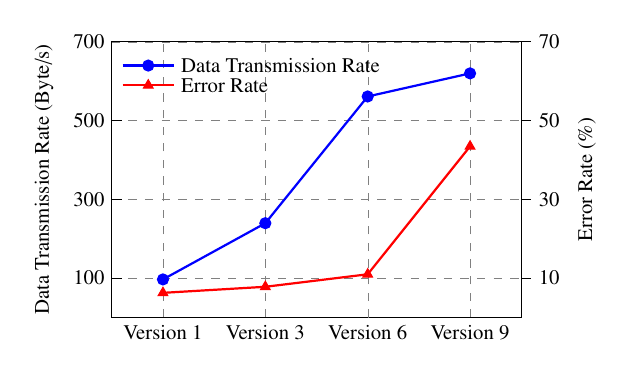
\begin{tikzpicture}[x = 1.3cm, y = 0.005cm]
        \tikzset{
            circle/.pic = {
                \draw[fill=blue, draw=blue] (0,0) circle (2pt);
            },
            triangle/.pic = {
                \draw[fill=red, draw=red] (90:2pt) -- (210:2pt) -- (-30:2pt) -- cycle;
            }
        }

        \draw[] (1,0) rectangle (5,700);
        % 在特定的刻度位置绘制虚线
        \foreach \x in {1, 2, 3, 4} {
            \draw[gray, ultra thin, dashed] (\x+0.5, 0) -- (\x+0.5, 700); % 在x轴的刻度位置绘制虚线
        }
        \foreach \y in {100, 300, 500, 700} {
            \draw[gray, ultra thin, dashed] (1, \y) -- (5, \y); % 在y轴的刻度位置绘制虚线
        }

        \foreach \y[count = \x] in {
            96.68, 239.35, 560.91, 619.54
        }{
            \coordinate (m-\x) at (\x+0.5,\y);
            \pic at (\x+0.5,\y) {circle};
            \node[above = 2pt, scale = .75] at (\x+0.5,\y) {};
        }
        \foreach \y[count = \x] in {
            6.26, 7.80, 10.97, 43.43
        }{
            \coordinate (n-\x) at (\x+0.5,\y*10);
            \pic at (\x+0.5,\y*10) {triangle};
            \node[below = 2pt, scale = .75] at (\x+0.5,\y*10) {};
        }
        
        \foreach \x[evaluate=\x as \y using \x+1] in {1,2,...,3} {
            \draw[blue, thick] (m-\x) -- (m-\y);
            \draw[red, thick] (n-\x) -- (n-\y);
        }
        \foreach \x[count = \xc] in {{Version 1},{Version 3},{Version 6},{Version 9}} {
            \node[below, scale = .75] at (\xc+0.5, 0) {\x};
            \draw[] (\xc+0.5, 0) --++ (0, .2);
        }

        % 绘制左侧y轴
        \foreach \y[count = \yc] in {100, 300, 500, 700} {
            \draw[] (1, \y) node[left, scale = .75] {\y} --++ (.1, 0);
        }

         % 绘制右侧y轴
        \draw (5, 0) -- (5, 700);
        \foreach \y in {10, 30, 50, 70} { % 对应红线数据范围的y刻度
            \draw (5, \y * 10) --++ (0.1, 0) node[right, scale = .75] {\y}; % 调整红线y刻度位置
        }
       
       \node[anchor = north west] at (1,700) {
        \tikz {
            \draw[blue, thick] (0.5,50) -- (1,50);
            \pic at (0.75,50) {circle};
            \node[anchor = west, scale = .75] at (1,50) {Data Transmission Rate
};
            \draw[red, thick] (0.5,0) -- (1,0);
            \pic at (0.75,0) {triangle};
            \node[anchor = west, scale = .75] at (1,0) {Error Rate};
        } };
        % 添加左侧坐标轴说明
        \node[rotate=90, anchor=south, scale = .75] at (0.5, 350) {Data Transmission Rate (Byte/s)};

        % % 添加右侧坐标轴说明
        \node[rotate=90, anchor=south, scale = .75] at (5.8, 350) {Error Rate (\%)};

    \end{tikzpicture}
    \caption{Comparison of Communication Performance with Different Versions of CQR Codes}
    \label{fig:qrcode_size_performance}
\end{figure}



\subsubsection{Impact of Display-Camera Angle and Distance on Communication Performance}
% 为评估CQR-UC在实际应用中的适应能力,实验分别测试了显示器-摄像头夹角和距离对通信性能的影响。实验由数据发送方向数据接收方发送8KB数据,记录通信的传输速率和误码率,每组实验重复5次。实验结果如图\ref{tab:angle_transmission}和图\ref{fig:distances}所示。

To evaluate the practical applicability of CQR-UC, we investigated how variations in the display-camera angle and distance affect communication performance. In each experiment, 8 KB of data were transmitted under different configurations, and both the data transmission rate and error rate were measured. Each configuration was tested five times. Results are detailed in Figure \ref{tab:angle_transmission} and Figure \ref{fig:distances}.

% 图\ref{tab:angle_transmission}所示为显示器-摄像头夹角对通信性能的影响。在较小的角度下(如\SI{0}{\degree}-\SI{10}{\degree}),CQR-UC表现出较高的数据传输速率和较低误码率。当夹角增加到\SI{15}{\degree}时,误码率大幅上升,导致数据传输速率显著下降。当摄像头与屏幕之间的夹角超过\SI{20}{\degree}时,由于误码率过高,通信双方无法建立连接。其主要原因为在过大显示器-摄像头夹角下,二维码在摄像头成像平面中出现严重的透视失真,模块几何形状从矩形变为梯形且模块分布不均匀,加之水下环境的光学干扰,接收端的解码算法难以正确对CQR code解码。
\begin{figure}[H] % 使用figure环境
\centering
    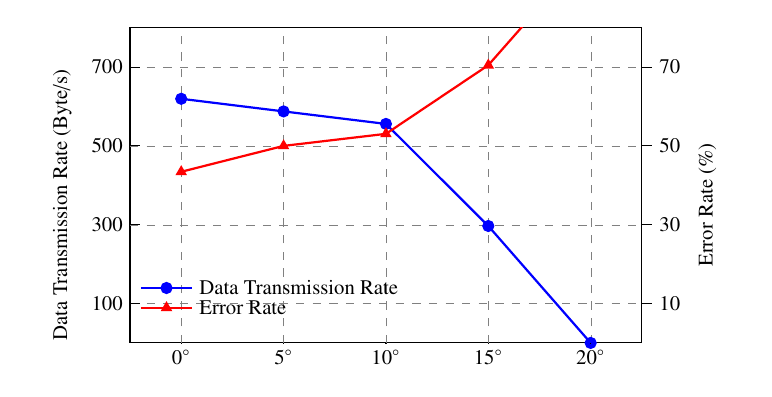
\begin{tikzpicture}[x = 1.3cm, y = 0.005cm]
        \tikzset{
            circle/.pic = {
                \draw[fill=blue, draw=blue] (0,0) circle (2pt);
            },
            triangle/.pic = {
                \draw[fill=red, draw=red] (90:2pt) -- (210:2pt) -- (-30:2pt) -- cycle;
            }
        }
        % 设置裁剪区域,使得超出此区域的内容不显示
        \clip (0,-65) rectangle (7,800);
        \draw[] (1,0) rectangle (6,800);
        % 在特定的刻度位置绘制虚线
        \foreach \x in {1, 2, 3, 4, 5} {
            \draw[gray, ultra thin, dashed] (\x+0.5, 0) -- (\x+0.5, 800); % 在x轴的刻度位置绘制虚线
        }
        \foreach \y in {100, 300, 500, 700} {
            \draw[gray, ultra thin, dashed] (1, \y) -- (6, \y); % 在y轴的刻度位置绘制虚线
        }

        \foreach \y[count = \x] in {
           619.54, 587.52, 555.77, 296.71, 0
        }{
            \coordinate (m-\x) at (\x+0.5,\y);
            \pic at (\x+0.5,\y) {circle};
            \node[above = 2pt, scale = .75] at (\x+0.5,\y) {};
        }
        \foreach \y[count = \x] in {
            43.43, 50.00, 53.06, 70.48, 100
        }{
            \coordinate (n-\x) at (\x+0.5,\y*10);
            \pic at (\x+0.5,\y*10) {triangle};
            \node[below = 2pt, scale = .75] at (\x+0.5,\y*10) {};
        }
        
        \foreach \x[evaluate=\x as \y using \x+1] in {1,2,...,4} {
            \draw[blue, thick] (m-\x) -- (m-\y);
            \draw[red, thick] (n-\x) -- (n-\y);
        }
        \foreach \x[count = \xc] in {{ \SI{0}{\degree}},{ \SI{5}{\degree}},{ \SI{10}{\degree}},{ \SI{15}{\degree}},{ \SI{20}{\degree}}} {
            \node[below, scale = .75] at (\xc+0.5, 0) {\x};
            \draw[] (\xc+0.5, 0) --++ (0, .2);
        }

        % 绘制左侧y轴
        \foreach \y[count = \yc] in {100, 300, 500, 700} {
            \draw[] (1, \y) node[left, scale = .75] {\y} --++ (.1, 0);
        }

         % 绘制右侧y轴
        \draw (6, 0) -- (6, 700);
        \foreach \y in {10, 30, 50, 70} { % 对应红线数据范围的y刻度
            \draw (6, \y * 10) --++ (0.1, 0) node[right, scale = .75] {\y}; % 调整红线y刻度位置
        }
       
       \node[anchor = north west] at (1,200) {
        \tikz {
            \draw[blue, thick] (0.5,50) -- (1,50);
            \pic at (0.75,50) {circle};
            \node[anchor = west, scale = .75] at (1,50) {Data Transmission Rate};
            \draw[red, thick] (0.5,0) -- (1,0);
            \pic at (0.75,0) {triangle};
            \node[anchor = west, scale = .75] at (1,0) {Error Rate};
        } };
        % 添加左侧坐标轴说明
        \node[rotate=90, anchor=south, scale = .75] at (0.5, 350) {Data Transmission Rate (Byte/s)};

        % % 添加右侧坐标轴说明
        \node[rotate=90, anchor=south, scale = .75] at (6.8, 350) {Error Rate (\%)};

    \end{tikzpicture}
    \caption{Comparison of Communication Performance at Different Display-camera Angles}
    \label{tab:angle_transmission}
\end{figure}

As shown in Figure~\ref{tab:angle_transmission}, the display-camera angle had a substantial impact on the performance of CQR-UC. The highest data transmission rates and lowest error rates were observed at small angles (\SI{0}{\degree}-\SI{10}{\degree}). However, performance deteriorated significantly at \SI{15}{\degree}, with a marked increase in error rate. 
Beyond \SI{20}{\degree}, communication failed because of severe perspective distortion and increased underwater optical interference, which prevented successful decoding of the CQR codes.



% 图\ref{fig:distances}显示了不同显示器-摄像头距离下CQR-UC的最优传输性能。从实验结果可知,随着距离的增加,系统的最优性能逐渐下降,同时所需二维码版逐步降低。在距离较小(20cm)时,较高版本的二维码(Version 9)可提供最优的传输速率;而在较大距离下(80cm),仅低版本二维码(Version 1)能够维持基本通信。当距离进一步增加时,由于信号强度、图像分辨率和水下环境干扰多重限制,通信双方无法有效建立连接。显示器-摄像头距离对性能的显著影响主要源于二维码模块在摄像头成像中的像素密度(像素每模块)随距离增加而迅速下降。较大显示器-摄像头距离导致单个模块在成像平面上的物理尺寸缩小,水下环境进一步导致二维码成像模糊,接收端难以接收到有效的CQR code。
\begin{figure}[!ht] % 使用figure环境
\centering
    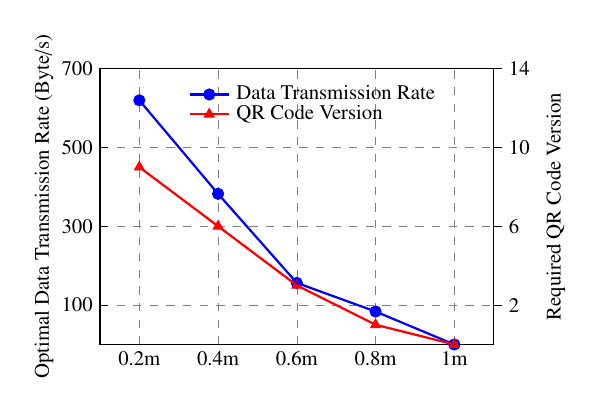
\begin{tikzpicture}[x = 1cm, y = 0.005cm]
        \tikzset{
            circle/.pic = {
                \draw[fill=blue, draw=blue] (0,0) circle (2pt);
            },
            triangle/.pic = {
                \draw[fill=red, draw=red] (90:2pt) -- (210:2pt) -- (-30:2pt) -- cycle;
            }
        }
        % 设置裁剪区域,使得超出此区域的内容不显示
        % \clip (0,-55) rectangle (7.5, 730);
        \draw[] (1,0) rectangle (6, 700);
        % 在特定的刻度位置绘制虚线
        \foreach \x in {1, 2, 3, 4, 5} {
            \draw[gray, ultra thin, dashed] (\x+0.5, 0) -- (\x+0.5, 700); % 在x轴的刻度位置绘制虚线
        }
        \foreach \y in {100, 300, 500} {
            \draw[gray, ultra thin, dashed] (1, \y) -- (6, \y); % 在y轴的刻度位置绘制虚线
        }

        \foreach \y[count = \x] in {
           619.54, 382.28, 156.23, 83.62, 0
        }{
            \coordinate (m-\x) at (\x+0.5,\y);
            \pic at (\x+0.5,\y) {circle};
            \node[above = 2pt, scale = .75] at (\x+0.5,\y) {} ;
        }
        \foreach \y[count = \x] in {
            9, 6, 3, 1, 0
        }{
            \coordinate (n-\x) at (\x+0.5,\y*50);
            \pic at (\x+0.5,\y*50) {triangle};
            \node[below = 2pt, scale = .75] at (\x+0.5,\y*50) {};
        }
        
        \foreach \x[evaluate=\x as \y using \x+1] in {1,2,...,4} {
            \draw[blue, thick] (m-\x) -- (m-\y);
            \draw[red, thick] (n-\x) -- (n-\y);
        }
        \foreach \x[count = \xc] in {{0.2m},{0.4m},{ 0.6m},{0.8m},{1m}} {
            \node[below, scale = .75] at (\xc+0.5, 0) {\x};
            \draw[] (\xc+0.5, 0) --++ (0, .2);
        }

        % 绘制左侧y轴
        \foreach \y[count = \yc] in {100, 300, 500, 700} {
            \draw[] (1, \y) node[left, scale = .75] {\y} --++ (.1, 0);
        }

         % 绘制右侧y轴
        \draw (6, 0) -- (6, 700);
        \foreach \y in {2, 6, 10, 14} { % 对应红线数据范围的y刻度
            \draw (6, \y * 50) --++ (0.1, 0) node[right, scale = .75] {\y}; % 调整红线y刻度位置
        }
       
       \node[anchor = north west] at (2.0,700) {
        \tikz {
            \draw[blue, thick] (0.5,50) -- (1,50);
            \pic at (0.75,50) {circle};
            \node[anchor = west, scale = .75] at (1,55) {Data Transmission Rate};
            \draw[red, thick] (0.5,0) -- (1,0);
            \pic at (0.75,0) {triangle};
            \node[anchor = west, scale = .75] at (1,0) {QR Code Version};
        } };
        % 添加左侧坐标轴说明
        \node[rotate=90, anchor=south, scale = .75] at (0.5, 350) { Optimal Data Transmission Rate (Byte/s)};

        % % 添加右侧坐标轴说明
        \node[rotate=90, anchor=south, scale = .75] at (7, 350) {Required QR Code Version};
    \end{tikzpicture}
    \caption{Comparison of Communication Performance at Different Distances}
    \label{fig:distances}
\end{figure}

Figure \ref{fig:distances} shows the optimal data transmission rate of CQR-UC at different display-camera distances. The experimental results revealed that as distance increased, both optimal performance and the required QR code version decreased in a stepwise manner. At 0.2m, Version 9 achieved the highest transmission rate, while at 0.8m, only Version 1 maintained basic communication. Beyond 0.8m, a stable connection could no longer be established. This is because a larger display-camera distance reduces the apparent size of each module in the captured image, significantly hindering accurate recognition by the receiver.




\subsubsection{Impact of Environments and Devices on Communication Performance}
% 实验评估了不同水环境和通信设备对CQR-UC通信性能的影响。实验选择了三种典型的水环境:海水、湖水和纯净水(分别代表了海洋、内陆水和理想水下通信环境)以及两种实验设备:平板电脑和树莓派(分别代表高性能通信设备和资源受限通信设备)。受屏幕大小限制,树莓派通信设备采用Version 1的二维码进行通信测试,而平板电脑则采用Version 9。实验结果如图\ref{fig:water} 所示。实验结果表明,在三种水环境中,两种通信设备表现出一致的趋势:纯净水环境中的通信性能最佳,其次是海水,湖水的通信性能最差。CQR-UC在海水和湖水中的通信速率比纯净水平均下降35\%和65\%。这种性能差异的主要原因在于三种水环境对光传播特性的不同影响:纯净水具有高透明度和低散射性,光吸收较少,因此二维码模块在摄像头成像中较为清晰,容易被接收方正确解码。海水较低的透明度和高盐度引起的散射效应会造成一定颜色失真。然而,在短距离通信条件下,数据增强模块可恢复大部分二维码的颜色。因此,在海水中CQR-UC仍可保持较高性能。湖水由于含有大量悬浮颗粒物(如藻类和泥沙),散射和吸收效应显著增强,造成二维码模块的对比度大幅降低,颜色严重失真,导致解码困难,因此通信性能因此显著下降。

Experiments assessed CQR-UC's performance across three environments, i.e. seawater, lake water, and purified water (simulating marine, inland, and ideal conditions), and using tablets (high-performance) and Raspberry Pi devices (resource-constrained). Raspberry Pi devices used Version 1 QR codes due to screen size, while tablets used Version 9. 
Figure \ref{fig:water} demonstrates consistent performance trends across all environments for both device types: communication performance is best in purified water, followed by seawater, and then lake water. 
Compared to purified water, data transmission rates decreased by an average of 35\% in seawater and 65\% in lake water. 
These differences were primarily attributable to the distinct light propagation characteristics of each environment. Purified water, with its high transparency and low scattering, minimized light absorption and enabled accurate CQR code decoding. Seawater, characterized by reduced transparency and salt-induced scattering, caused some color distortion. However, our image enhancement largely mitigated this issue, maintaining relatively high communication performance. In contrast, lake water, which contained abundant suspended particles, exhibited significantly stronger scattering and absorption. This resulted in substantial reductions in CQR code contrast and severe color distortion, leading to markedly degraded communication performance.

% 此外,实验结果还表明,通信设备的硬件性能对系统的通信表现具有显著影响。平板电脑由于具有更大的屏幕、更高的摄像头分辨率和更强的数据处理能力,在所有环境中通信性能均优于树莓派设备。相比之下,树莓派设备受限于较小的屏幕尺寸、较低的摄像头分辨率以及较弱的数据处理能力,仅能支持低版本二维码,从而在数据传输速率上表现出较大的局限性。尤其是在复杂水环境(如湖水)中,树莓派设备的性能受环境干扰影响更为显著。尽管树莓派设备的通信性能较低,但其具有小型化、低成本和便携性的特点,这使其在某些特定应用场景中具有重要价值。例如,在水下设备近距离维护和水下传感器数据收集等场景中,通信距离较短且对传输速率的需求相对较低,树莓派设备能够以较低的成本实现可靠的数据传输。此外,其低功耗特性也有助于延长设备的运行时间,从而满足对能耗敏感的水下应用需求。值得注意的是,我们仅对CQR-UC进行了初步实现,其通信性能仍有较大提升空间。

Furthermore, the results indicate that hardware capabilities have a substantial impact on communication performance. Owing to their larger screens, higher camera resolution, and faster processing speeds, tablets consistently outperformed Raspberry Pi devices in data transmission rates across all environments. In contrast, the Raspberry Pi's hardware limitations necessitated the use of lower-version QR codes, significantly constraining transmission rates, particularly in challenging environments such as lake water. Nevertheless, the Raspberry Pi device remains advantageous for specific use cases due to its compact size, low cost, and portability.  It enables reliable, low-cost data transmission in short-range, low-bandwidth underwater applications, such as equipment maintenance and sensor data collection. Its low power consumption further extends operating duration in energy-constrained underwater environments. Notably, the current implementation of CQR-UC is still preliminary and offers substantial potential for future optimization.

\begin{figure}[!tb]
\centering
	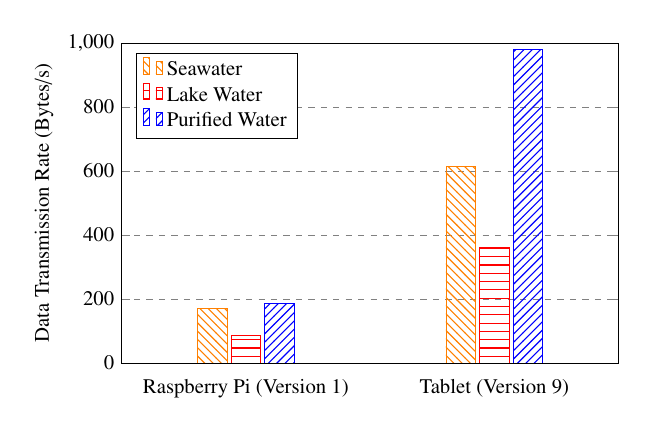
\begin{tikzpicture}[scale=0.75]
		\begin{axis}
			[
                width=10cm, % 显式设置宽度
			height=7cm, % 保持适当高度
			ybar,					% 柱状图
			bar width=0.5cm,		% 柱子宽度
			xtick={1, 2},			% 设置x轴的具体刻度点
			ytick distance=200,		% y的刻度距离
			xmin=0.5, xmax=2.5,		% x的范围
			ymin=0, ymax=1000,		% y的范围
			legend pos=north west,	% 图例的位置
                legend style={align=left,
                cells={anchor=west},}, % 图例文本左对齐
			ylabel={Data Transmission Rate (Bytes/s)},	% Y轴标签
			xticklabels={Raspberry Pi (Version 1), Tablet (Version 9)},  % X轴的标签
                 xtick style={draw=none}, % 取消X轴的刻度线
			ymajorgrids,			% 显示y轴刻度的网格线
			grid style={thin, gray, dashed},
			]
			\addlegendentry{Seawater}
			\addplot+ [pattern=north west lines, pattern color=orange, draw=orange] coordinates {(1,170) (2,613)};		% 橙色反斜线
			\addlegendentry{Lake Water}
			\addplot+ [pattern=horizontal lines, pattern color=red] coordinates {(1,85) (2,362)};		% 红色水平线
                \addlegendentry{Purified Water}
			\addplot+ [pattern=north east lines, pattern color=blue, draw=blue] coordinates {(1,185) (2,980)};		% 蓝色斜线
		\end{axis}
	\end{tikzpicture}
		\caption{
		Comparison of Data Transmission rates across Different Water Types and Devices
	}
	\label{fig:water}
\end{figure}

\subsection{Performance Evaluation of CQR-GAN}
% 为验证CQR-GAN对CQR code图像的增强的效果,我们训练了不同的图像增强模型,并测试它们在单色二维码和不同通道的CQR code上的图像增强效果。实验利用相同数据集训练UW-CNN~\cite{sun2018transferring},U-net~\cite{ronneberger2015u},CycleGAN以及CQR-GAN模型,实验结果如图\ref{fig:com_schemes}所示。其中None表示没有图像增强模块。

To evaluate the enhancement capabilities of CQR-GAN for underwater CQR code images, we trained and compared it with UW-CNN~\cite{sun2018transferring}, U-Net~\cite{ronneberger2015u}, CycleGAN~\cite{zhu2020cyclegan} and MSFFT-Net~\cite{WU2025MSFFT} using the same dataset. Figure \ref{fig:com_schemes} presents the image enhancement performance of these models on monochrome QR codes and multi-channel CQR codes in underwater environment. "None" indicates the absence of image enhancement.

\begin{figure}[h]
\centering
	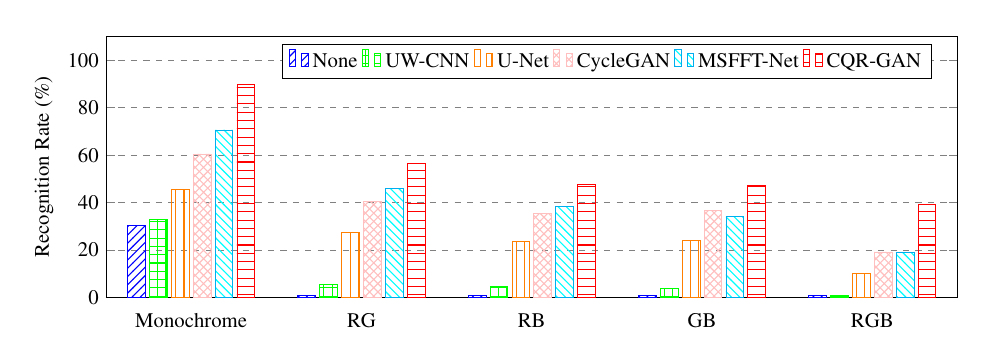
\begin{tikzpicture}[scale=0.75]
		\begin{axis}[
			ybar,					% 柱状图
			bar width=0.3cm,		% 柱子宽度
			xtick={1,2,3,4,5},		% 设置x轴的具体刻度点
			ytick distance=20,		% y的刻度距离
			xmin=0.5, xmax=5.5,		% x的范围
			ymin=0, ymax=110,		% y的范围
			legend pos=north east,	% 图例的位置
                legend style={align=left, legend columns=-1}, % 图例文本左对齐且水平显示
			ylabel={Recognition Rate (\%)},	% Y轴标签
			xticklabels={Monochrome, RG, RB, GB, RGB},  % X轴的标签
                xtick style={draw=none}, % 取消X轴的刻度线
			ymajorgrids,			% 显示y轴刻度的网格线
			grid style={thin, gray, dashed},
                width=16cm,				% 设置图形的宽度
			height=6cm,				% 设置图形的高度
		]
		\addlegendentry{None}
		\addplot+ [pattern=north east lines, pattern color=blue] coordinates {(1,30.5) (2,1) (3,1) (4,1) (5,1)};		% 蓝色斜线

            \addlegendentry{UW-CNN}
            \addplot+ [pattern=grid, pattern color=green, draw=green] coordinates {(1,32.8) (2,5.5) (3,4.45) (4,3.98) (5,1)};		% 绿色水平线

            \addlegendentry{U-Net}
            \addplot+ [pattern=vertical lines, pattern color=orange,draw=orange] coordinates {(1,45.5) (2,27.36) (3,23.6) (4,24.02) (5,10.3)};		% 绿色水平线

            \addlegendentry{CycleGAN}
            \addplot+ [pattern=crosshatch, pattern color=pink,draw=pink] coordinates {(1,60.5) (2,40.61) (3,35.35) (4,36.54) (5,19.2)};		% 绿色水平线

            % \addlegendentry{CQR-GAN w/o attention}
            % \addplot+ [pattern=dots, pattern color=cyan,draw=cyan] coordinates {(1,67.35) (2,45.20) (3,41.21) (4,42.51) (5,28.53)};		% 绿色水平线

            \addlegendentry{MSFFT-Net}
    			\addplot+ [pattern=north west lines, pattern color=cyan,draw=cyan] coordinates {(1,70.62) (2,45.86) (3,38.36) (4,34.03) (5,19.08)};% 青色斜线

            \addlegendentry{CQR-GAN}
			\addplot+ [pattern=horizontal lines, pattern color=red,draw=red] coordinates {(1,89.63) (2,56.57) (3,47.82) (4,47.42) (5,39.06)};		% 红色水平线
            
		\end{axis}
	\end{tikzpicture}
	\caption{Comparison of Underwater QR Code Recognition Performance across Different Image Enhancement Models}
	\label{fig:com_schemes}
\end{figure}

% 在没有图像增强模块的情况下,只有30.5\%的单色二维码能够被正确识别,且所有CQR code均无法识别。这主要归因于水下环境对二维码图像的强烈干扰,导致解码算法难以有效解码二维码。尽管UW-CNN和U-Net模型在一定程度上能够还原水下二维码图像,但其效果仍然有限。CycleGAN通过引入Cycle Consistency Loss和对抗训练机制,实现了水下二维码到normal二维码的图像风格转换,还原了部分颜色信息,取得了较一定的增强效果。在所有方法中,CQR-GAN展现了最佳的图像增强性能。CQR-GAN在CycleGAN中引入了局部判别机制,使得生成的CQR code图像在细粒度上与真实图像的域分布一致,有效还原了水下CQR code图像的真实颜色。图\ref{fig:enter-label6}所示为二维码的图像增强效果示例。可以观察到,增强后的单色二维码和CQR code图像在颜色亮度和模块对比度上均有显著改善,模块边界更加清晰,具有更高的可辨识性。

Without image enhancement, only 30.5\% of monochrome QR codes were recognized, and no CQR codes could be decoded, as underwater interference severely impaired decoding accuracy. While UW-CNN and U-Net provided limited improvements, CycleGAN, leveraging cycle consistency and adversarial training, partially restored colors and yielded moderate gains. MSFFT-Net, a state-of-the-art model originally designed for enhancing underwater natural scenes, also achieved relatively good recognition rates but tended to introduce color distortions when applied to underwater QR code images. CQR-GAN achieved the best enhancement performance by incorporating a patch-based strategy into the CycleGAN framework. This allowed it to maintain fine-grained consistency with real images and effectively restore the true colors of underwater CQR codes. As shown in Figure~\ref{fig:enter-label6}, the enhanced QR codes exhibit improved color brightness, higher module contrast, and clearer module boundaries, resulting in significantly better recognizability.

\begin{figure}[H]
\centering
    \includegraphics[width=0.9\linewidth]{enhanced_picture.pdf}
    \caption{Example of Image Enhancement Results for QR Code}
    \label{fig:enter-label6}
\end{figure}


\subsection{Ablation Study}
% 为评估 QR-GAN中各个策略(分块增强、循环一致性、自特征保持)对模型识别性能的贡献,我们在三种2通道水下CQR code(RG、RB、GB)上设计了以下消融对比:
% 1)取消图像分块增强(w/o Patch);2)取消循环一致性损失(w/o CYC);3)取消自特征保持损失(w/o SFP)。
% 图\ref{fig:ablation_comparison}展示了完整模型与三种消融版本在RG、RB、GB三种2通道上水下CQR code上的识别率对比结果。
% 在所有情况下,完整CQR-GAN均取得了最优性能。当消除了分块增强或者循环一致性损失时,模型性能大幅下降(低于30\%),这表明局部细节与信息保持对CQR code增强至关重要。当消除自特征保持损失时(o/w SFP),模型对水下CQR code的识别率在RG、RB 和GB上分别下降了8.7\%,2.6\% 和 3.5\%,这验证了自特征保持损失在保持CQR code纹理和颜色一致性上的有效性。

To evaluate the contribution of patch-based strategy, self-feature preservation loss and cycle-consistency loss to CQR recognition performance, we conducted ablation studies on 2-channel underwater CQR codes (RG, RB, GB) by removing each strategy individually: (1) without patch-based strategy (w/o Patch); (2) without cycle-consistency loss (w/o CYC); (3) without self-feature preservation loss (w/o SFP).
Figure \ref{fig:ablation_comparison} presents the CQR code recognition rates of CQR-GAN and these ablation variants.
CQR-GAN consistently achieved the highest performance. 
Removing patch-based strategy or cycle-consistency loss significantly reduced model performance (below 30\%), highlighting the importance of local details and information preservation. Removing self-feature preservation loss decreased the recognition rate by 8.7\%, 2.6\%, and 3.5\% on RG, RB, and GB channel CQR codes, respectively, validating its effectiveness in maintaining CQR code texture and color consistency.

\begin{figure}[h]
  \centering
  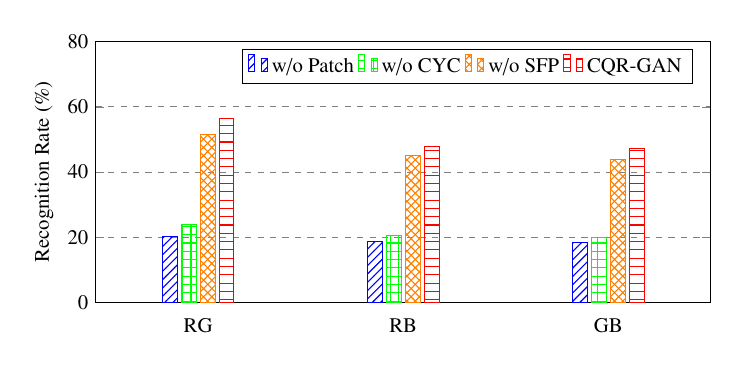
\begin{tikzpicture}[scale=0.75]
    \begin{axis}[
      ybar,
      bar width=0.25cm,
      xtick={1,2,3},
      ytick distance=20,
      xmin=0.5, xmax=3.5,
      ymin=0, ymax=80,
      legend pos=north east,	% 图例的位置
      legend style={align=left, legend columns=-1},
      ylabel={Recognition Rate (\%)},
      xticklabels={RG, RB, GB},
      ymajorgrids,
      xtick style={draw=none}, % 取消X轴的刻度线
      grid style={thin, gray, dashed},
      width=12cm,
      height=6cm,
    ]
      % 各模型图例(去掉 w/o Local)
      \addlegendentry{w/o Patch}
      \addplot+ [pattern=north east lines, pattern color=blue, draw=blue]
        coordinates {(1,20.27) (2,18.74) (3,18.56)};
      \addlegendentry{w/o CYC}
      \addplot+ [pattern=grid, pattern color=green, draw=green]
        coordinates {(1,23.82) (2,20.45) (3,20.13)};
      \addlegendentry{w/o SFP}
      \addplot+ [pattern=crosshatch, pattern color=orange, draw=orange]
        coordinates {(1,51.63) (2,45.23) (3,43.93)};
      \addlegendentry{CQR-GAN}
      \addplot+ [pattern=horizontal lines, pattern color=red, draw=red]
        coordinates {(1,56.57) (2,47.82) (3,47.42)};
    \end{axis}
  \end{tikzpicture}
  \caption{Performance Comparison of CQR-GAN Ablation Variants on 2-channel Underwater CQR Codes}
  \label{fig:ablation_comparison}
\end{figure}


\section{Discussion}
\subsection{Advantages of CQR-UC over Traditional Underwater Communication Methods}
% 相比于传统水下通信方法,CQR-UC在成本、便携性和环境适应性方面具有优势。水声通信设备昂贵,难以推广应用,然而CQR-UC成本很低,以树莓派实现的水下通信设备成本甚至低于40\$;电磁通信功耗高、设备体积大,CQR-UC功耗低,设备体积较小,可以安装在小型水下设备中,尤其是以树莓派实现的水下CQR code通信设备。传统水下光通信依赖昂贵的专业光学设备,部署和维护复杂。相比之下,CQR-UC方法利用普通显示器和摄像头实现了低成本的水下连续可靠通信。此外,CQR-UC系统结构简单、功耗低、便于部署,尤其适合潜水员或小型水下机器人与水下设备间的近距离通信、水下传感器数据收集等场景,能够满足短距离、实时性和高可靠性通信需求。

CQR-UC offers several advantages over traditional underwater communication methods, including compact size, low cost, low power consumption, and ease of deployment and maintenance. For instance, acoustic communication equipment is typically expensive, whereas CQR-UC provides a low-cost alternative---Raspberry Pi devices can cost less than \$40. Compared to power-hungry and bulky electromagnetic communication systems, CQR-UC operates at low power (under 15W) and features a compact design ideal for small underwater devices. Moreover, unlike specialized and costly optical communication systems, CQR-UC utilizes commonly available displays and cameras for reliable, continuous communication. These advantages make it particularly well-suited for some specialized applications, such as short-range underwater equipment maintenance and sensor data collection by divers/small robots.

\subsection{Comparison with Traditional CQR code-based communication}
% 传统CQR code通信方法主要针对空气环境设计,应用于水下环境将面临一些挑战。首先,水下环境的光吸收和散射效应会导致CQR code的color distortion and low contrast,从而显著降低CQR code的识别率。其次,传统方法通常缺乏双向可靠通信机制,不适合大量连续数据交互。针对上述问题,CQR-UC方法进行了专门优化。一方面,CQR-UC引入了CQR-GAN深度神经网络,用于CQR code图像的颜色还原与对比度增强,有效补偿了水下光学干扰,显著提升了CQR code的识别率。另一方面,CQR-UC设计了一种轻量化高效的专用通信协议,能够支持数据的连续可靠传输,且能够适用于水下高噪声环境和性能受限的水下通信设备。

Traditional CQR code-based communication, which is primarily designed for use in air, encounters significant challenges when applied in underwater environments. These challenges are primarily due to the effects of light absorption and scattering in water, which result in color distortion and low contrast, thereby hindering recognition of CQR codes. 
Furthermore, the lack of continuous reliable communication protocol limits large-scale data interaction. To address these limitations, CQR-UC optimizes CQR code-based communication for underwater scenarios. It employs a CQR-GAN model to enhance CQR code images, effectively mitigating optical interference and improving recognition accuracy. In addition, CQR-UC employs CUP, a lightweight and reliable communication protocol specifically designed to support continuous data transmission under underwater conditions.

\subsection{Theoretical Maximum Data Transmission Rate}
% 通信速率是评价水下通信系统性能的关键指标,为进一步给出QR-UC方法的通信性能上限,我们从理论上分析了CQR-UC通信的最大速率。假设水下通信设备的显示器大小和摄像头分辨率满足CQR code显示和采集要求,且CQR code的显示时延远小于其识别时延,则CQR code的理论最大通信速率$S_{max}$可表示为Eq.~\ref{eq10}。

To evaluate underwater communication performance, we theoretically derive the maximum data transmission rate $S_{max}$ of the CQR-UC, representing its performance upper bound. Assuming adequate display size and camera resolution for CQR code presentation and capture, and considering display latency to be negligible compared to recognition latency, $S_{max}$ is defined as:
\begin{equation}
    S_{max}=min(F_{DIS}, F_{CAM}/2, F_{REC})\times D_\rho(L_{ECL}) \times C_{color} \times D_{qr} (v)\times ACC
    \label{eq10}
\end{equation}
% 其中,$F_{DIS}$为显示器的刷新频率,$F_{CAM}$为摄像头的采集频率,$F_{IDE}$为CQR code识别频率(二维码识别时延的倒数)。$D_\rho$为单通道二维码的信息密度,其为纠错等级$L_{ECC}$和编码方案$S$的函数。$C_{color}$表示CQR code采用的颜色通道的数量,$D_{qr}$为单通道CQR code的数据容量,其为二维码版本$v$的函数。$ACC$为CQR code识别准确率。根据奈奎斯特采样定理,为保证摄像头能够无失真地采集到显示的CQR code图像,$F_{CAM}$至少需为$F_{LCD}$的2倍~\cite{JIANG2016colorful}。在CQR code方案($D_\rho$,$C_{color}$和$D_{qr}$确定)和$ACC$确定的情况下,理论最大通信速率将由$F_{LCD}$、$F_{CAM}/2$和$F_{IDE}$的最小值决定。
Here, $F_{DIS}$ is the display refresh rate, $F_{CAM}$ is the camera capture rate, and $F_{REC}$ represents the CQR code recognition rate, defined as the inverse of the recognition latency.
$D_\rho$ represents the information density of a single-channel QR code, which depends on error correction level $L_{ECL}$. $C_{color}$ is the number of color channels used, and $D_{qr}$ is the data capacity of a single-channel CQR code, determined by the QR code version $v$. $ACC$ is the recognition accuracy. 
According to the Nyquist sampling theorem,  $F_{CAM}$ must be at least twice $F_{DIS}$ to ensure accurate capture of CQR code images~\cite{JIANG2016colorful}. Therefore, for a fixed CQR code scheme (i.e., fixed $D_\rho$, $C_{color}$, and $D_{qr}$) and a given $ACC$, the theoretical maximum data transmission rate is constrained by the minimum of $F_{DIS}$, $F_{CAM}/2$, and $F_{REC}$.

\section{Conclusion}
% 本文针对水下无线通信设备昂贵、功耗高且便携性差的问题,提出了一种基于CQR code的水下无线通信方法CQR-UC。本文构建了基于CQR code的水下无线通信框架,并针对水下CQR code识别率低的问题,设计了基于生成对抗网络的CQR code图像增强模型CQR-GAN。此外,本文设计了水下CQR code通信专用协议CUP,实现了水下环境中数据的连续可靠传输。实验验证了CQR-UC在多种水下环境适应性和性能。CQR-UC为小型自主水下机器人及其他水下设备间的低成本、短距离通信提供了一种高效可靠的解决方案。下一步研究将优化CQR-UC的性能和鲁棒性。在性能方面,将构建更完备和高效的数据集,提高CQR-GAN模型识别准确率;在通信鲁棒性方面,研究应用深度学习模型还原畸变的CQR code图像,以应对远距离通信和屏幕-摄像头夹角过大和引起的二维码图像失真问题,提升CQR-UC在复杂水下环境中通信鲁棒性。
To address the challenges of high cost, high power consumption, and limited portability in existing underwater wireless communication systems, this paper presents CQR-UC, a novel underwater communication method based on CQR codes. CQR-UC establishes an underwater communication framework based on CQR codes and employs CQR-GAN model to improve the recognition accuracy in underwater environments. In addition, a dedicated underwater communication protocol, CUP, is designed to ensure continuous and reliable bidirectional data transmission. Experimental results demonstrate the efficacy and performance of CQR-UC across various underwater environments. Given its compact design, low cost, and low power consumption, CQR-UC holds strong potential for practical applications such as short-range underwater equipment maintenance and sensor data collection.

%%%%%%%%%%%%%%%%%%%%%%%%%%%%%%%%%%%%%%%%%%

%%%%%%%%%%%%%%%%%%%%%%%%%%%%%%%%%%%%%%%%%%
%% optional
%\supplementary{The following supporting information can be downloaded at:  \linksupplementary{s1}, Figure S1: title; Table S1: title; Video S1: title.}

% Only for journal Methods and Protocols:
% If you wish to submit a video article, please do so with any other supplementary material.
% \supplementary{The following supporting information can be downloaded at: \linksupplementary{s1}, Figure S1: title; Table S1: title; Video S1: title. A supporting video article is available at doi: link.}

% Only for journal Hardware:
% If you wish to submit a video article, please do so with any other supplementary material.
% \supplementary{The following supporting information can be downloaded at: \linksupplementary{s1}, Figure S1: title; Table S1: title; Video S1: title.\vspace{6pt}\\
%\begin{tabularx}{\textwidth}{lll}
%\toprule
%\textbf{Name} & \textbf{Type} & \textbf{Description} \\
%\midrule
%S1 & Python script (.py) & Script of python source code used in XX \\
%S2 & Text (.txt) & Script of modelling code used to make Figure X \\
%S3 & Text (.txt) & Raw data from experiment X \\
%S4 & Video (.mp4) & Video demonstrating the hardware in use \\
%... & ... & ... \\
%\bottomrule
%\end{tabularx}
%}

%%%%%%%%%%%%%%%%%%%%%%%%%%%%%%%%%%%%%%%%%%


% Only for journal Nursing Reports
%\publicinvolvement{Please describe how the public (patients, consumers, carers) were involved in the research. Consider reporting against the GRIPP2 (Guidance for Reporting Involvement of Patients and the Public) checklist. If the public were not involved in any aspect of the research add: ``No public involvement in any aspect of this research''.}

% Only for journal Nursing Reports
%\guidelinesstandards{Please add a statement indicating which reporting guideline was used when drafting the report. For example, ``This manuscript was drafted against the XXX (the full name of reporting guidelines and citation) for XXX (type of research) research''. A complete list of reporting guidelines can be accessed via the equator network: \url{https://www.equator-network.org/}.}

% Only for journal Nursing Reports
%\useofartificialintelligence{Please describe in detail any and all uses of artificial intelligence (AI) or AI-assisted tools used in the preparation of the manuscript. This may include, but is not limited to, language translation, language editing and grammar, or generating text. Alternatively, please state that “AI or AI-assisted tools were not used in drafting any aspect of this manuscript”.}

%%%%%%%%%%%%%%%%%%%%%%%%%%%%%%%%%%%%%%%%%%
%% Optional

%% Only for journal Encyclopedia
%\entrylink{The Link to this entry published on the encyclopedia platform.}
%\textbf{Author Contributions: }{Conceptualization, Z.Z. and Y.F.; methodology, Z.Z., Y.F.; software, Y.F., S.L.; validation, Y.F. and Q.Z.; formal analysis, Y.F., Z.Z. and Q.Z.; investigation, Z.Z. and Y.F.; data curation, Y.F. and S.L.; writing---original draft preparation, Y.F., X.F.; writing---review and editing, Z.Z., Q.Z., X.F., w.c. and Q.M.; visualization, Y.F. and S.L; supervision, X.F.; funding acquisition, Q.Z., Q.M. All authors have read and agreed to the published version of the manuscript.}

\section*{Acknowledgements}
This research was supported by grants from the National Natural Science Foundation of China (62002056) and the Fundamental Research Funds for Public Universities in Liaoning.

%\textbf{Conflicts of Interest:}{The authors declare that they have no known competing financial interests or personal relationships that could have appeared to influence the work reported in this paper.}
%%%%%%%%%%%%%%%%%%%%%%%%%%%%%%%%%%%%%%%%%%





\section*{Appendix A}
The CQR code object detection model employs Yolov5-Lite, which was trained on a dataset comprising 1500 monochrome QR code images and 1500 CQR code images from each of three environments: seawater, lake water, and purified water. QR code bounding box annotations are included. The dataset is split into training and validation sets with an 8:2 ratio, and the model is trained for 300 epochs.

\section*{Appendix B}
\setcounter{table}{0} % 重新从A1开始编号
\renewcommand{\thetable}{B.\arabic{table}}

% CCS(CQR code Encoding Scheme)占4 bits,其中the first bit为1表示通信中的数据帧采用monochrome QR code, 否则为CQR code。第2-4 bit对应CQR code采用的GRB颜色通道。具体CQR code Encoding Scheme如表\ref{tab:ccs}所示。

The 4-bit CCS uses the first bit to indicate whether data frames are transmitted using monochrome QR codes (1) or CQR codes (0). The remaining three bits (bits 2-4) specify the GRB color channels used in CQR codes. Table \ref{tab:ccs} provides details on the CCS.

\begin{table}[H]
\centering
\caption{CQR Code Encoding Scheme of CUP}
\begin{tabular}{ c c c c }
\hline
Value& Channel Number & Channels Used & Color of CQR Code \\ \hline
1000  & - & - & Black and White  \\ 
0110  & 2 & RG & Red, Green, Yellow, Black  \\ 
0011  & 2  & GB & Green, Blue, Cyan, Black  \\ 
0101  & 2  & RB & Red, Blue, Magenta, Black  \\
\multirow{3}{*}{0111} & \multirow{3}{*}{3} & \multirow{3}{*}{RGB} & \parbox[t]{4.3cm}{\centering Red, Green, Blue, Yellow, Cyan, Magenta, Black, White} \\ 
\hline
\end{tabular}
\label{tab:ccs}
\end{table}

\section*{Appendix C}
% Status Code占2 bit。CUP协议规定通信包括4种状态,如表\ref{tab:status}所示。
% Status code=0表示通信双方处于连接请求状态。在该状态下,通信双方进行连接请求、连接响应以及参数协商(CQR code Encoding Scheme、压缩等级)。
% Status code=1表示发送的数据已被接收者不完整接收。在该状态下,接收者通知发送者缺失的帧,发送者重传缺失帧。
% Status code=2表示发送的数据已被接收者完整接收。在该状态下,接收者通知发送者完成数据传输,发送者响应完成数据传输。
% Status code=3表示连接终止。在该状态下,通信双方关闭通信连接,释放资源,并进入连接请求状态。

% The 2-bit Status Code in the CUP protocol defines four communication states as shown in Table \ref{tab:status}.
% \begin{itemize}
% \item 0 (Connection Request): The two communicating parties perform connection requests, acknowledges, and parameter negotiation (CQR code encoding scheme and compression level).
% \item 1 (Incomplete Reception): Receiver requests retransmission of missing frames from the sender.
% \item 2 (Complete Reception): Receiver requests connection termination.
% \item 3 (Connection Termination): The two communicating parties close the connection, release resources, and return to the Connection Request state.
% \end{itemize}

The 2-bit Status Code in the CUP protocol defines four communication states. Status 0, known as Connection Request, initiates connection setup, handling acknowledgments and negotiating parameters like CQR code encoding scheme and compression level. Status 1, Incomplete Reception, indicates the receiver has detected missing frames and requests their retransmission. Status 2, Complete Reception, signifies that all frames have been successfully received, prompting a request for connection termination. Status 3, Connection Termination, closes the connection, releases resources, and resets both parties to the Connection Request state.

% \begin{table}[h]
% \caption{Status Code of CUP}
% \begin{tabular}{ c c c c }
% \hline
% Value of Status Code & Status  &  Communication Stage & Action  \\ \hline
% \multirow{2}{*}{0}  & \multirow{2}{*}{\centering Connection Request} & \multirow{2}{*}{\centering Communication Establishment} & \multirow{2}{*}{\centering Connection Request, Connection Response, Parameter Negotiation}  \\ 
% \multirow{2}{*}{1}  & \multirow{2}{*}{\centering Incomplete Reception} & \multirow{2}{*}{\centering Data Transmission} & \multirow{2}{*}{\centering Missing Frame Retransmission}  \\ 
% \multirow{2}{*}{2}  & \multirow{2}{*}{\centering Complete Reception}  & \multirow{2}{*}{\centering Communication Termination} & \multirow{2}{*}{\centering Data Transmission End Notification and Response}  \\ 
% \multirow{2}{*}{3}  & \multirow{2}{*}{\centering Connection Termination} & \multirow{2}{*}{\centering Communication Termination} & \multirow{2}{*}{\centering Release Resources, Enter Connection Request} \\ \hline
% \end{tabular}
% \label{tab:status}
% \end{table}


% \begin{table}[h]
% \centering
% \caption{Status code of CUP}
% \begin{tabular}{ c c c}
% \hline
% Value & Status & Action  \\ \hline
% \multirow{2}{*}{0} & \multirow{2}{*}{Connection Request} & \parbox[t]{6.5cm} {\centering Connection Request and Acknowledge, Parameter Negotiation}  \\ 
% 1  & Incomplete Reception & Missing Frame Retransmission  \\ 
% 2  & Complete Reception  & Data Transmission End Notification \\ 
% 3  & Connection Termination  & Connection termination, Connection Request Initiation\\ \hline
% \end{tabular}
% \label{tab:status}
% \end{table}

\section*{Appendix D}
% Compress占2 bit。CUP协议规定通信可采用4个压缩等级,如表\ref{tab:compression}所示。压缩等级0表示不对数据进行压缩。压缩等级1-3分别表示采用DEFLATE压缩算法的~\cite{oswal2016deflate}3,6,9等级压缩。在实际应用中,可根据实际传输数据类别和传输任务选择不同的压缩等级。

The 2-bit Compress in the CUP protocol specifies four compression levels. Level 0 indicates no compression. Level 1-3 correspond to DEFLATE Compression~\cite{oswal2016deflate} levels 3, 6, and 9, respectively. The appropriate compression level should be selected based on data type and transmission requirements.

% \begin{table}[H]
% \centering
% \caption{Compression level of CUP (DEFLATE means corresponding DEFLATE compression level)}
% \begin{tabular}{ c c c}
% \hline
% Value & DEFLATE &  Application Scenario  \\ \hline
% 0    & 0 &  Small amount of data transfers or no compression needed   \\ 
% 1    & 3 & Time-sensitive compression   \\ 
% 2    & 6 & Standard underwater communication with good compression \\ 
% 3    & 9 & Poor communication conditions and low compression time priority \\ \hline
% \end{tabular}
% \label{tab:compression}
% \end{table}

%% If you have bib database file and want bibtex to generate the
%% bibitems, please use
%%
%%  \bibliographystyle{elsarticle-num} 
%%  \bibliography{<your bibdatabase>}

%% else use the following coding to input the bibitems directly in the
%% TeX file.

%% Refer following link for more details about bibliography and citations.
%% https://en.wikibooks.org/wiki/LaTeX/Bibliography_Management

\bibliographystyle{elsarticle-num}
\bibliography{ref}
\end{document}

\endinput
%%
%% End of file `elsarticle-template-num.tex'.
